\documentclass{kjpaper}
\usepackage[authoryear,sort&compress,round]{natbib}
\bibliographystyle{abbrvnat}
\usepgfplotslibrary{groupplots}
\usetikzlibrary{positioning,arrows.meta,fit}
% ---- project macros ----
\newcommand{\sname}{PRISM-Loc}
\newcommand{\code}[1]{\texttt{#1}}
\newcommand{\T}{\top}
\title{\sname: Three LiDAR Localization Backends Behind One ROS~2 Contract, with Middleware-Free Estimator Cores}
\correspondingauthor{kangjmo91@gmail.com}
\paperurl{https://github.com/kjungmo/prism\string_loc}
\author[1]{Jungmo Kang}
\affil[1]{Independent Researcher, Seoul, Republic of Korea}
\keywords{mobile robots, LiDAR localization, Monte Carlo localization, NDT, error-state Kalman filter, ROS~2}
\setlength{\emergencystretch}{2em}
\begin{document}
\begin{abstract}
Widely used open-source tools for map-based LiDAR localization of mobile robots are still largely organized by sensor suite: a 2D scanner typically calls for an AMCL-style particle filter over an occupancy grid, a 3D LiDAR for an NDT-based tracker over a point-cloud map, and an inertial- or GNSS-aided platform for a Kalman fusion node, often with different topics, parameters, initialization, and recovery behavior. Existing libraries already share one particle-filter core across 2D and 3D sensor models, and other systems already relocalize a robot by branch-and-bound scan matching. We describe \emph{\sname}, an open-source ROS~2 localization stack that places three established estimator families behind one node contract: \code{laser2d}, a likelihood-field Monte Carlo localizer; \code{ndt3d}, a planar NDT-MCL backend \citep{saarinen2013ndtmcl} that reuses the same particle filter with a Gaussian-voxel measurement model; and \code{fusion3d}, a 15-state error-state Kalman filter fusing LiDAR, IMU, and RTK-GNSS. Every backend publishes the same \code{map}$\to$\code{odom} transform and pose with covariance and accepts the same \code{/initialpose} seeding, all filter mathematics live in Eigen-only C++17 cores that are tested without a ROS runtime, and \code{laser2d} relocalizes a kidnapped robot on request (at startup or by a service call) by deterministic branch-and-bound scan matching over a map-sized search window restricted to cells not marked occupied, keeping the top-$K$ candidate poses and committing one only after several odometry-chained scans concentrate a normalized heuristic evidence score on it, and otherwise reporting the place as ambiguous. We claim no new estimator theory and no new verification principle; the contribution is this particular integration, released as software. In seeded closed-loop experiments on \emph{synthetic} data that drive the actual cores, the 2D tracker holds a steady-state mean position error of 0.105\,m, branch-and-bound relocalization succeeds on 97 of 100 kidnapped-robot queries in a 6\,m room with zero false accepts at its default threshold, on 40\,m and 80\,m maps with repeated structure the single-scan rule accepts a wrong pose on 6 and 15 of 120 queries, which multi-scan verification reduces to 0 and 1 of 120 (pooled 95\% Wilson interval 0.1--2.3\%) while committing as many correct poses (242 against 241 of 300), and the ESKF bounds a 10\,s aiding dropout to 0.125\,m RMSE, although a 100-run NEES test shows that its covariance is overconfident (full-state NEES above the 95\% interval at 89 of 120 epochs, mainly in attitude; bias blocks consistent). No external baseline and no real or public data are used, and no field-accuracy claim is made. Code: \url{https://github.com/kjungmo/prism_loc}.
\end{abstract}

\maketitle
\section{Introduction}\label{sec:intro}

% overview.tex -- architecture teaser (TikZ), ported from docs/paper/figures/fig_architecture.tex
\begin{figure}[t]
\centering
\footnotesize
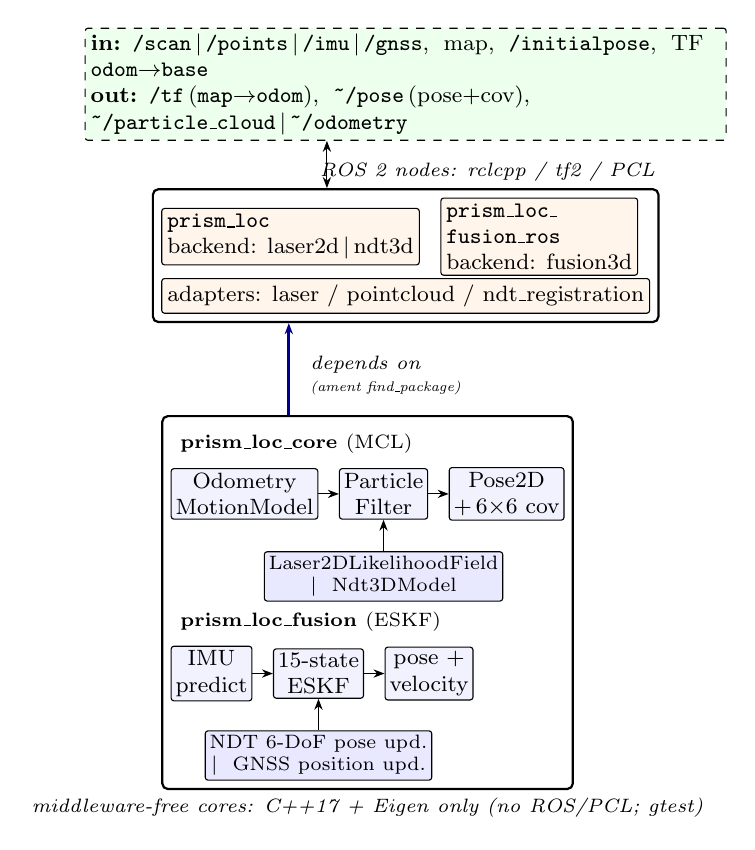
\begin{tikzpicture}[
  font=\footnotesize,
  >={Stealth[length=1.4mm]},
  node distance=2mm and 2.6mm,
  block/.style={draw, rounded corners=1pt, inner sep=1.6pt, align=center,
                minimum height=4.4mm},
  core/.style={block, fill=blue!5},
  meas/.style={block, fill=blue!9, font=\scriptsize},
  ros/.style={block, fill=orange!8, align=left, inner sep=2pt},
  io/.style={draw, dashed, rounded corners=1pt, inner sep=2pt, align=left,
             fill=green!7, text width=80mm},
  flow/.style={->, thin},
]

% ============ Estimator core layer (bottom) ============
% ---- prism_loc_core (MCL) ----
\node[core] (omm) {Odometry\\MotionModel};
\node[core, right=of omm] (pf) {Particle\\Filter};
\node[core, right=of pf] (mclout) {Pose2D\\$+\,6{\times}6$ cov};
\node[meas, below=4mm of pf] (mcM)
  {Laser2DLikelihoodField\\$\mid$~~Ndt3DModel};
\draw[flow] (omm) -- (pf);
\draw[flow] (pf) -- (mclout);
\draw[flow] (mcM) -- (pf);
\node[font=\scriptsize\bfseries, anchor=south west]
  (mcllbl) at ([yshift=0.6mm]omm.north west) {prism\_loc\_core \textmd{(MCL)}};

% ---- prism_loc_fusion (ESKF) ----
\node[core, below=16mm of omm.south west, anchor=north west] (imu) {IMU\\predict};
\node[core, right=of imu] (eskf) {15-state\\ESKF};
\node[core, right=of eskf] (fusout) {pose $+$\\velocity};
\node[meas, below=4mm of eskf] (esM)
  {NDT 6-DoF pose upd.\\$\mid$~~GNSS position upd.};
\draw[flow] (imu) -- (eskf);
\draw[flow] (eskf) -- (fusout);
\draw[flow] (esM) -- (eskf);
\node[font=\scriptsize\bfseries, anchor=south west]
  (fuslbl) at ([yshift=0.6mm]imu.north west) {prism\_loc\_fusion \textmd{(ESKF)}};

% fit box around the core layer
\node[draw, thick, rounded corners=2pt, fill=none,
      fit=(mcllbl)(mclout)(mcM)(imu)(fusout)(esM),
      inner sep=3pt] (corebox) {};
\node[anchor=north, font=\scriptsize\itshape, inner sep=1.5pt]
  at ([yshift=-0.4mm]corebox.south)
  {middleware-free cores: C++17 + Eigen only \textmd{(no ROS/PCL; gtest)}};

% ============ ROS 2 node layer (top) ============
\node[ros, above=19mm of corebox.north west, anchor=south west]
  (plnode) {\texttt{prism\_loc}\\backend: laser2d\,$\mid$\,ndt3d};
\node[ros, right=of plnode]
  (fnode) {\texttt{prism\_loc\_}\\\texttt{fusion\_ros}\\backend: fusion3d};
\node[ros, below=1.6mm of plnode.south west, anchor=north west]
  (adapt) {adapters: laser / pointcloud / ndt\_registration};
\node[draw, thick, rounded corners=2pt, fill=none,
      fit=(plnode)(fnode)(adapt), inner sep=3pt] (rosbox) {};
\node[anchor=south east, font=\scriptsize\itshape, inner sep=1.5pt]
  at ([yshift=0.2mm]rosbox.north east)
  {ROS~2 nodes: \textmd{rclcpp / tf2 / PCL}};

% dependency arrow: nodes consume cores upward
\draw[->, very thick, blue!55!black]
  ([xshift=-10mm]corebox.north) -- ([xshift=-10mm]corebox.north |- rosbox.south);
\node[text=black, font=\scriptsize\itshape, align=left, anchor=west]
  at ([xshift=-8.5mm, yshift=5mm]corebox.north)
  {depends on\\\textmd{\tiny(ament find\_package)}};

% ============ Shared contract I/O (top) ============
\node[io, above=6mm of rosbox.north, anchor=south] (io) {%
  \textbf{in:} \texttt{/scan}\,$\mid$\,\texttt{/points}\,$\mid$\,\texttt{/imu}\,$\mid$\,\texttt{/gnss},\;
  map,\; \texttt{/initialpose},\; TF \texttt{odom}$\to$\texttt{base}\\
  \textbf{out:} \texttt{/tf}\,(\texttt{map}$\to$\texttt{odom}),\;
  \texttt{\char`~/pose}\,(pose+cov),\;
  \texttt{\char`~/particle\_cloud}\,$\mid$\,\texttt{\char`~/odometry}};
\draw[<->, thin]
  ([xshift=-10mm]rosbox.north) -- ([xshift=-10mm]rosbox.north |- io.south);

\end{tikzpicture}
\caption{\textbf{\sname{} overview.} Two middleware-free estimator cores (bottom, C++17 + Eigen only): \code{prism\_loc\_core} runs the MCL loop (\textsc{OdometryMotionModel}\,$\to$\,\textsc{ParticleFilter}, corrected by either the \textsc{Laser2DLikelihoodField} or the \textsc{Ndt3DModel} measurement model, plus a branch-and-bound relocalizer), and \code{prism\_loc\_fusion} runs a 15-state ESKF (IMU prediction, corrected by NDT 6-DoF pose and GNSS position updates). The ROS~2 node packages (top) consume the cores upward through ament, select a backend at launch, bridge messages through adapters, and expose one shared contract: a \code{map}$\to$\code{odom} TF, a pose-with-covariance output, and an \code{/initialpose} seed input.}
  \label{fig:overview}
\end{figure}


Localizing a mobile robot against a prior map is, on paper, a solved problem, but the widely used open-source tools are still largely organized by sensor suite. A team fielding a 2D LiDAR typically reaches for \code{nav2\_amcl}, a particle filter that tracks a planar pose against an occupancy grid and nothing else. A team with a 3D LiDAR may reach instead for an \code{hdl\_localization}-style tracker built around 3D NDT registration \citep{koide2019portable}. A team that must fuse inertial and satellite measurements may reach for a \code{robot\_localization}-style node \citep{moore2014generalized}, which composes an EKF over odometry, IMU, and GNSS but leaves the map-relative LiDAR measurement to another node. These tools differ in topic interface, parameter vocabulary, initialization, and recovery behavior, so a practitioner who moves from a 2D platform to a 3D one, or who adds a GNSS receiver, must re-integrate much of the localization layer.

The split is not universal, and several efforts reduce it. The survey of the ROS~2 navigation maintainers \citep{macenski2023survey} catalogs the shortcomings of AMCL and reports a proposed design for a localization framework that builds 2D and 3D localization systems from modular components. Beluga \citep{puga2024beluga,ekumen2022belugarepo} is a ROS-agnostic C++17 Monte Carlo localization library whose ROS~2 nodes offer interface parity with \code{nav2\_amcl} and pair one particle-filter core with likelihood-field and 2D and 3D NDT sensor models; Autoware's pose-estimator arbiter \citep{autoware2024arbiter} launches several heterogeneous pose estimators and provides a mechanism to stop and resume them; and fuse \citep{locus2018fuse} and MOLA \citep{blancoclaraco2025mola} provide modular estimation frameworks. How a stack initializes, degrades, and recovers also matters in deployment: the Nav2 marathon deployment \citep{macenski2020marathon} names low localization confidence as one of the two causes behind most of its recovery triggers. Classical MCL recovers from such failures through stochastic mechanisms, random particle injection or dual sampling \citep{fox1999efficient,thrun2001robust}, which are hard to reproduce in a test; later systems add failure detection \citep{akai2023reliable}, keep several particle populations seeded by map matching \citep{garcia2023mhamcl}, or reset a tracker from a branch-and-bound global search \citep{koide2021hdlgl,sasaki2026globalloc}.

We describe \emph{\sname}, an engineering integration that packages three map-based LiDAR localization backends behind one ROS~2 node contract (\Cref{fig:overview}): \code{laser2d}, a 2D likelihood-field Monte Carlo localizer against an occupancy grid; \code{ndt3d}, a 3D NDT-MCL backend \citep{saarinen2013ndtmcl} that reuses the same particle filter with a voxel-Gaussian measurement model over a prior point cloud, sampling the planar $(x,y,\theta)$ pose; and \code{fusion3d}, a 15-state error-state Kalman filter (ESKF) that fuses 3D LiDAR, IMU, and RTK-GNSS with IMU-bias estimation. All three present the same interface, a \code{map}$\to$\code{odom} transform, a pose with $6\times6$ covariance on a private \code{\char`~/pose} topic that differs between the two nodes only by namespace and can be remapped (\Cref{tab:contract}), and \code{/initialpose} seeding, so choosing between a 2D scan, a 3D cloud, and an inertial/GNSS-aided configuration is a launch-time choice of parameter or launch file rather than a change of interface. We claim no new estimator theory: likelihood-field MCL, NDT-MCL, ESKF fusion, and branch-and-bound scan matching are all established, and so are the broader patterns we use, namely one particle-filter core shared by 2D and 3D measurement models \citep{puga2024beluga,ekumen2022belugarepo}, branch-and-bound relocalization against a prior map \citep{hess2016realtime,koide2021hdlgl}, and tracking several global-localization hypotheses over time until the ambiguity is resolved \citep{gao2019global,garcia2023mhamcl}. We are not aware of a released package that combines exactly the three backends below behind one contract with a relocalizer that can decline to commit; that combination is the contribution, delivered as usable open-source software. \Cref{tab:positioning} lists the closest prior work for each component.
\begin{itemize}
  \item \emph{One Pluggable Contract}: three estimator families (2D likelihood-field MCL, 3D NDT-MCL, and LiDAR+IMU+RTK-GNSS ESKF fusion) present one ROS~2 \code{map}$\to$\code{odom} contract, so the sensor suite selects a backend, not a stack with a different interface. Beluga already serves its likelihood-field and NDT particle filters through one node interface \citep{puga2024beluga,ekumen2022belugarepo}; the addition here is an inertial/GNSS Kalman backend that shares the same \code{map}$\to$\code{odom} TF edge, pose message type, and \code{/initialpose} seeding (\code{laser2d} and \code{ndt3d} are chosen by one \code{backend} parameter, \code{fusion3d} by its own launch file); its covariance is overconfident in our test, so we release it as experimental (\Cref{sec:disc}). The release adds fail-fast configuration checks, a startup watchdog that names the input that has gone silent, and a single-source parameter reference.
  \item \emph{Middleware-Free, Deterministic Cores}: all filter mathematics sit behind an Eigen-only boundary with no \code{rclcpp}, \code{tf2}, or PCL, and all sampling routes through one seeded generator, so every algorithmic claim is exercised by 63 deterministic unit and integration tests and by closed-loop synthetic experiments that compile the cores directly. Middleware-independent estimator cores are established practice \citep{puga2024beluga,pedrosa2019lama}; we list this as a property of the artifact, not as a research contribution.
  \item \emph{Global Relocalization That Can Abstain}: for \code{laser2d}, the branch-and-bound correlative scan matcher of \citet{hess2016realtime}, run over a max-pooled likelihood pyramid, finds candidate poses for a kidnapped robot from one scan and re-seeds the MCL particle set once a candidate is verified, in place of stochastic random-injection recovery. By the standard branch-and-bound argument of \citet{hess2016realtime}, restated for our search set in \Cref{sec:bbs}, the search returns the best correlative score over the non-occupied (free or unknown) cells of the rotation--translation lattice; this is the discrete optimum of a surrogate score, not an optimal pose estimate. The search window is sized from the map, so the search is global up to a configurable compute cap (100\,m per axis by default). Because the optimum of one scan can be a look-alike place, the node keeps the top-$K$ distinct candidates, propagates each by odometry and re-scores it by a local branch-and-bound match, and commits one only when it holds most of a normalized heuristic evidence score over several scans, reporting the place as ambiguous otherwise. Tracking several hypotheses \citep{gao2019global,garcia2023mhamcl} and requiring evidence to persist over several scans and some motion before declaring a robot localized \citep{adurthi2023scan} are established, and concurrent work makes an abstaining decision explicit for LiDAR-to-BIM initialization \citep{zhang2026movefirst}; what is specific here is this combination on 2D occupancy grids, wired to re-seed the shared MCL core.
\end{itemize}

We validate \sname{} at the level of correctness and closed-loop behavior, not field accuracy. On seeded synthetic worlds generated to match the filters' assumptions, the \code{laser2d} tracker holds a steady-state mean position error of 0.105\,m while KLD-adaptive resampling shrinks the particle set from the 2000-particle ceiling to the 500-particle floor; branch-and-bound relocalization recovers 97 of 100 kidnapped-robot queries in a 6\,m room under up to 80\% beam clutter with zero false accepts at its default acceptance threshold, and on 40\,m and 80\,m maps recovers 50 and 41 of 60 poses that lie outside the fixed window of our first release, which recovered 2 and 0; there, however, a single scan accepts a wrong pose on 6 and 15 of 120 queries because repeated shelves look alike, and multi-scan verification brings this to 0 and 1 of 120 without losing correct fixes overall; and the ESKF limits a 10\,s loss of all aiding to 0.125\,m position RMSE, while a 100-run Monte Carlo NEES test shows that its covariance is overconfident, mainly in attitude. These numbers demonstrate that the assembled pipelines behave as intended; they are not a benchmark. We run no external baseline and use no real or public data, so we make no claim of accuracy or robustness relative to \code{nav2\_amcl}, Beluga, MH-AMCL, or the global-localization methods of \Cref{sec:related}; that comparison is planned (\Cref{sec:disc}).

\section{Related Work}\label{sec:related}

\noindent\textbf{Monte Carlo Localization.}
Particle-filter localization was introduced by \citet{dellaert1999montecarlo} and \citet{fox1999efficient}, who represent the pose posterior as a weighted sample set updated by motion-model prediction, sensor-likelihood weighting, and resampling, and who demonstrated global localization from a uniform prior on real robots. \citet{thrun2001robust} later hardened MCL against accurate sensors and the kidnapped-robot problem via Mixture-MCL's dual sampler, and \citet{fox2003kld} made the sample size adaptive through KLD-sampling; the odometry motion model and likelihood-field sensor model we use are the textbook forms of \citet{thrun2005probabilistic}. The particle-filter core of \sname{} is a direct descendant of this line and of its \code{nav2\_amcl} lineage; we contribute no new filter theory. What differs is factoring: the same predict--weight--resample core is shared, unchanged, between a 2D likelihood-field backend and a 3D NDT backend, and recovery is delegated to a deterministic branch-and-bound search (\Cref{sec:bbs}) rather than stochastic injection or dual sampling.

\noindent\textbf{NDT Representations and Measurement Models.}
\citet{biber2003ndt} introduced the Normal Distributions Transform, modeling a scan as per-cell Gaussians and reducing registration to Newton optimization of a smooth score; \citet{magnusson2007scan} generalized the representation to 3D voxel grids for field deployment on mining vehicles. Both use NDT for deterministic scan-to-scan or scan-to-map registration that requires a reasonable initial guess. The \code{ndt3d} backend of \sname{} adopts the Gaussian-voxel representation but reads the NDT score out as a per-particle likelihood inside the shared MCL core (NDT-MCL rather than NDT registration), trading the quadratic convergence of Newton alignment for the multi-hypothesis robustness of the particle filter, so the 2D and 3D backends differ only in their measurement model.

\noindent\textbf{LiDAR-Inertial Fusion and Robot Software Systems.}
\citet{sola2017quaternion} is the mathematical basis of the \code{fusion3d} backend: the nominal/error-state decomposition, local angular-error parameterization, and predict--correct--inject--reset cycle are implemented essentially as derived there. On the systems side, \citet{moore2014generalized} established the configurable EKF/UKF fusion node for ROS, \citet{wan2018robust} demonstrated an industrial ESKF fusing GNSS-RTK, LiDAR, and IMU at centimeter accuracy as a production system tied to its own pre-built LiDAR maps, and Nav2 \citep{macenski2020marathon} treats localization as an external, swappable component. Tightly-coupled LiDAR-inertial odometry such as FAST-LIO \citep{xu2021fastlio}, and applied 3D map-based tracking systems \citep{koide2019portable}, are complementary: they produce ego-motion and maps, whereas \sname{} localizes within a prior map. Relative to these, \sname{} places three known estimator families behind one ROS~2 topic and TF contract, each implemented as a library that is unit-testable without a middleware runtime, a property that \code{robot\_localization}'s otherwise modular design did not prioritize, and which answers the modular-localization framework that \citet{macenski2023survey} left as future work.

\noindent\textbf{Global (Kidnapped-Robot) Localization.}
\citet{olson2009correlative} formulated 2D scan matching as exhaustive correlative search over a rasterized log-likelihood table with coarse-to-fine multi-resolution pruning, and \citet{hess2016realtime} bounded that search with branch-and-bound over a precomputed grid pyramid to run loop closure in real time inside Cartographer. \sname{} borrows exactly this branch-and-bound-over-pyramid primitive but applies it in a narrower setting: relocalization against a known static map, with no submaps or pose graph to maintain, whose verified result re-seeds the particle filter in place of the heuristic recovery of classical MCL \citep{fox1999efficient,thrun2001robust}.

\section{\sname: One Localization Contract over Three Middleware-Free Estimators}\label{sec:method}

\sname{} separates \emph{what} a localization node promises its consumers from \emph{how} a pose is estimated. We first state the estimation problem and the output contract shared by all backends, then describe the two-layer architecture that realizes the contract (\Cref{sec:arch}), the shared particle-filter core (\Cref{sec:mcl}), its two measurement models (\Cref{sec:meas}), the branch-and-bound relocalizer (\Cref{sec:bbs}), the error-state fusion filter (\Cref{sec:eskf}), and the initialization and diagnostic layer (\Cref{sec:init}). Every equation below is transcribed from the C++ sources listed in \Cref{app:codemap}.

\noindent\textbf{Problem Setup: One Contract, Interchangeable Estimators.}
Let $m$ be a prior map (an occupancy grid or a point cloud), $\mathbf{u}_{1:t}$ the odometry or inertial inputs, and $\mathbf{z}_{1:t}$ the exteroceptive measurements (2D scans, 3D clouds, GNSS fixes). Each backend $b\in\mathcal{B}=\{\code{laser2d},\code{ndt3d},\code{fusion3d}\}$ approximates the Bayes-filter belief over the robot state $\mathbf{x}_t$ \citep{thrun2005probabilistic},
\begin{equation}\label{eq:bayes}
  \mathrm{bel}_b(\mathbf{x}_t) \;=\; \eta\, p_b(\mathbf{z}_t \mid \mathbf{x}_t, m) \int p_b(\mathbf{x}_t \mid \mathbf{u}_t, \mathbf{x}_{t-1})\, \mathrm{bel}_b(\mathbf{x}_{t-1})\, \mathrm{d}\mathbf{x}_{t-1},
\end{equation}
with a particle set for the two MCL backends and a Gaussian error state for \code{fusion3d}. Whatever the representation, a backend reports a point estimate $\hat{\mathbf{T}}_{\mathrm{map,base}}$ with a $6\times6$ covariance $\hat{\boldsymbol{\Sigma}}_t$ and, so as not to fight the odometry source that owns \code{odom}$\to$\code{base\_link}, broadcasts only the correction transform
\begin{equation}\label{eq:mapodom}
  \hat{\mathbf{T}}_{\mathrm{map,odom}} \;=\; \hat{\mathbf{T}}_{\mathrm{map,base}} \oplus \mathbf{T}_{\mathrm{odom,base}}^{-1},
\end{equation}
where $\oplus$ is pose composition and $\mathbf{T}_{\mathrm{odom,base}}$ is read from TF at the measurement stamp. \Cref{eq:mapodom} guarantees the round trip $\hat{\mathbf{T}}_{\mathrm{map,odom}}\oplus\mathbf{T}_{\mathrm{odom,base}}=\hat{\mathbf{T}}_{\mathrm{map,base}}$, which ROS-free unit tests assert to $10^{-9}$ on $SE(2)$ and $SE(3)$. The design objective is that the tuple (TF edge, pose topic, seeding topic) is identical for all $b\in\mathcal{B}$, so that the sensor suite, not the software stack, selects $b$.

\subsection{Separating Estimators from Middleware: Two Layers, One Contract}\label{sec:arch}

\sname{} is organized as two layers realized by four packages (\Cref{fig:overview}). The lower layer holds the estimator cores: \code{prism\_loc\_core} implements the MCL family and the relocalizer, and \code{prism\_loc\_fusion} implements the ESKF. Both are plain C++17 libraries whose only third-party dependency is Eigen; each \code{CMakeLists.txt} links \code{Eigen3::Eigen} alone, with no reference to \code{rclcpp}, \code{tf2}, or PCL. The upper layer holds the ROS~2 node packages \code{prism\_loc} (the \code{laser2d} and \code{ndt3d} backends, selected by a \code{backend} string parameter) and \code{prism\_loc\_fusion\_ros} (the \code{fusion3d} backend). Only these depend on the middleware, and the dependency direction is strictly upward.

The split buys three properties. First, \emph{unit-testability without a running graph}: each core builds and tests with a plain toolchain and GoogleTest, and continuous integration exercises this ROS-free path directly. Second, \emph{determinism}: all sampling routes through a single seeded \code{std::mt19937\_64} wrapper (ROS parameter \code{seed}, default 42), so a prediction, weighting, or resampling step is reproducible bit for bit, which makes the core tests assertable rather than merely statistical. Third, \emph{one output contract} (\Cref{tab:contract}): every backend broadcasts \code{map}$\to$\code{odom} per \Cref{eq:mapodom}, publishes a \code{PoseWithCovarianceStamped} on \code{\char`~/pose}, and accepts \code{/initialpose}; the MCL nodes add a particle cloud and the fusion node an \code{Odometry} message. Thin adapters convert \code{LaserScan}, \code{OccupancyGrid}, \code{PointCloud2}, and \code{.pcd} files into core value types, and in \code{fusion3d} an adapter wraps PCL's NDT registration to turn a live cloud into a 6-DoF pose measurement, so PCL appears only inside adapters. QoS profiles follow publisher semantics: sensor streams are subscribed with \code{SensorDataQoS} (best-effort), while the occupancy grid is subscribed \code{transient\_local} and \code{reliable} so the single latched map from \code{map\_server} reaches a late-joining node.

\begin{table}[t]
\centering
\caption{\textbf{Per-backend topic contract.} All backends additionally subscribe \code{/initialpose} and the TF \code{odom}$\to$\code{base\_link}, and broadcast \code{map}$\to$\code{odom} by \Cref{eq:mapodom} with the stamp future-dated by \code{transform\_tolerance} (default 0.1\,s). The private topic \code{\char`~/pose} resolves under the node name (\code{/prism\_loc/pose} for \code{laser2d} and \code{ndt3d}, \code{/prism\_loc\_fusion/pose} for \code{fusion3d}) and can be remapped.}\label{tab:contract}
\small
\begin{tabularx}{\linewidth}{@{}l>{\raggedright\arraybackslash}X>{\raggedright\arraybackslash}X>{\raggedright\arraybackslash}X@{}}
\toprule
Backend & Estimator core & Inputs & Outputs \\
\midrule
\code{laser2d} & MCL + likelihood field (\Cref{eq:laser}) & \code{/scan}, \code{/map} (\code{OccupancyGrid}) & \code{\char`~/pose}, \code{\char`~/particle\_cloud} \\
\code{ndt3d} & MCL + NDT score (\Cref{eq:ndt}) & \code{/points}, \code{.pcd} map file & \code{\char`~/pose}, \code{\char`~/particle\_cloud} \\
\code{fusion3d} & 15-state ESKF (\Cref{eq:eskfpred,eq:eskfupd}) & \code{/points}, \code{/imu}, \code{/gnss} (\code{NavSatFix}), \code{.pcd} map file & \code{\char`~/pose}, \code{\char`~/odometry} \\
\bottomrule
\end{tabularx}
\end{table}


\subsection{Sampling and Weighting Particles: One MCL Core for 2D and 3D}\label{sec:mcl}

Both pose-tracking backends share one particle filter over the planar pose $\mathbf{x}=(x,y,\theta)$ (\code{Pose2D}), with belief $\{(\mathbf{x}^{[i]}_t,w^{[i]}_t)\}_{i=1}^{N_t}$. The recursion is the one wired in \code{localization\_node.cpp} and summarized in \Cref{alg:mcl}.

\noindent\textbf{Motion Model.} \code{OdometryMotionModel} implements the sampling form of the odometry model \citep{thrun2005probabilistic}. Consecutive odometry poses are decomposed into $(\delta_{r1},\delta_t,\delta_{r2})$, with $\delta_{r1}=0$ whenever $\delta_t<10^{-3}$\,m (pure-rotation guard), and each particle is advanced by the noise-corrupted increment
\begin{equation}\label{eq:motion}
\begin{aligned}
\hat{\delta}_{r1} &= \delta_{r1} - \varepsilon\big(\alpha_1 \delta_{r1}^2 + \alpha_2 \delta_{t}^2\big), \qquad
\hat{\delta}_{r2} = \delta_{r2} - \varepsilon\big(\alpha_1 \delta_{r2}^2 + \alpha_2 \delta_{t}^2\big),\\
\hat{\delta}_{t}  &= \delta_{t}  - \varepsilon\big(\alpha_3 \delta_{t}^2 + \alpha_4(\delta_{r1}^2 + \delta_{r2}^2)\big),
\end{aligned}
\end{equation}
where $\varepsilon(\sigma^2)$ draws zero-mean Gaussian noise of variance $\sigma^2$ and $\alpha_{1..4}$ are the \code{alpha1}--\code{alpha4} parameters.

\noindent\textbf{Weighting.} Given a measurement model with log-likelihood $\ell(\mathbf{x})$ (\Cref{sec:meas}), the \code{correct} step of \code{ParticleFilter} replaces each weight by
\begin{equation}\label{eq:weights}
  w^{[i]} \;=\; \frac{\exp\!\big(\ell(\mathbf{x}^{[i]})-\ell_{\max}\big)}{\sum_{j}\exp\!\big(\ell(\mathbf{x}^{[j]})-\ell_{\max}\big)}, \qquad \ell_{\max}=\max_j \ell(\mathbf{x}^{[j]}),
\end{equation}
subtracting the per-step maximum for numerical stability. The weights are overwritten rather than multiplied into the previous ones; this coincides with the standard recursion after every resampling step (which leaves uniform weights), and otherwise discards the previous step's weights, a simplification we note rather than hide.

\noindent\textbf{KLD-Adaptive Resampling.} Resampling is triggered only when the effective sample size $N_{\mathrm{eff}}=(\sum_i w^{[i]})^2/\sum_i (w^{[i]})^2$ falls below $\tau N$ (\code{resample\_threshold} $\tau=0.5$). Samples are then drawn with probability proportional to weight and dropped into a histogram with bins of \code{kld\_bin\_xy} in $(x,y)$ and \code{kld\_bin\_yaw} in $\theta$. Following \citet{fox2003kld}, after $k>1$ distinct bins have been occupied the target sample count is
\begin{equation}\label{eq:kld}
  M_k \;=\; \frac{k-1}{2\,\epsilon_{\mathrm{kld}}}\left(1-\frac{2}{9(k-1)}+\sqrt{\frac{2}{9(k-1)}}\;z_{1-\delta}\right)^{3},
\end{equation}
and drawing stops once $n\ge\max(M_k,N_{\min})$ or $n=N_{\max}$, with $\epsilon_{\mathrm{kld}}$ (\code{kld\_err}), $z_{1-\delta}$ (\code{kld\_z}), and $[N_{\min},N_{\max}]$ (\code{min\_particles}, \code{max\_particles}) as parameters. The resampled set receives uniform weights.

\noindent\textbf{Pose Estimate.} The reported pose is the weighted mean of $(x,y)$ with the circular mean of $\theta$,
\begin{equation}\label{eq:estimate}
  \hat{x}=\textstyle\sum_i w^{[i]}x^{[i]},\quad \hat{y}=\sum_i w^{[i]}y^{[i]},\quad \hat{\theta}=\operatorname{atan2}\!\big(\sum_i w^{[i]}\sin\theta^{[i]},\,\sum_i w^{[i]}\cos\theta^{[i]}\big),
\end{equation}
and the $6\times6$ covariance carries the weighted planar second moments in $(x,y)$ and $\theta$, while $z$, roll, and pitch are marked unobserved with variance $10^{6}$.

\begin{algorithm}[t]
\caption{One \code{laser2d}/\code{ndt3d} filter update, as wired in \code{localization\_node.cpp}}\label{alg:mcl}
\KwIn{particle set $\mathcal{X}$; previous and current odometry poses $\mathbf{o}_{t-1},\mathbf{o}_t$; measurement model $\ell$; gates $d_{\min},a_{\min}$}
\If{$\|\mathbf{o}_t-\mathbf{o}_{t-1}\|_{xy}\ge d_{\min}$ \textbf{or} $|\theta(\mathbf{o}_t)-\theta(\mathbf{o}_{t-1})|\ge a_{\min}$ \textbf{or} a re-seed forced an update}{
  \For{$i\gets1$ \KwTo $|\mathcal{X}|$}{
    $\mathbf{x}^{[i]}\gets$ sample \Cref{eq:motion} from $(\mathbf{o}_{t-1},\mathbf{o}_t)$ applied to $\mathbf{x}^{[i]}$\;
  }
  compute weights $w^{[i]}$ by \Cref{eq:weights}\;
  \If{$N_{\mathrm{eff}}<\tau|\mathcal{X}|$}{
    $\mathcal{X}\gets$ KLD-resample until $n\ge\max(M_k,N_{\min})$ (\Cref{eq:kld}) or $n=N_{\max}$\;
  }
  $\mathbf{o}_{t-1}\gets\mathbf{o}_t$\;
}
\KwOut{$(\hat{x},\hat{y},\hat{\theta})$ and covariance by \Cref{eq:estimate}; $\hat{\mathbf{T}}_{\mathrm{map,odom}}$ by \Cref{eq:mapodom}}
\end{algorithm}

\subsection{Scoring Observations: Likelihood-Field and NDT Measurement Models}\label{sec:meas}

A backend differs from the other only through a \code{MeasurementModel}, whose single virtual method returns the unnormalized log-likelihood $\ell(\mathbf{x})$ of the current observation given a candidate base pose.

\noindent\textbf{2D Likelihood Field.} \code{Laser2DLikelihoodField} is the likelihood-field model \citep{thrun2005probabilistic}. At construction the occupancy grid (cells with value $\ge50$ occupied) is converted into a field $d(\cdot)$ holding the Euclidean distance to the nearest occupied cell, computed exactly by the separable squared-distance transform of \citet{felzenszwalb2012distance} and clamped at \code{likelihood\_max\_dist}. For a scan with ranges $r_j$ at bearings $\phi_j$, the model visits every $s$-th beam, $s=\max(1,\lfloor n/\code{max\_beams}\rfloor)$, discards ranges outside $(r_{\min},r_{\max})$, and scores
\begin{equation}\label{eq:laser}
  \ell_{\mathrm{2D}}(\mathbf{x}) \;=\; \sum_{j\in\mathcal{J}} \log\max\!\Big(z_{\mathrm{hit}}\exp\!\big(-d(\mathbf{e}_j(\mathbf{x}))^2/2\sigma_{\mathrm{hit}}^2\big) + z_{\mathrm{rand}}/r_{\max},\; 10^{-12}\Big),
\end{equation}
where $\mathbf{e}_j(\mathbf{x})$ is the beam endpoint $r_j(\cos\phi_j,\sin\phi_j)$ transformed into the map through $\mathbf{x}$ composed with the sensor mounting pose.

\noindent\textbf{3D NDT Score.} \code{Ndt3DModel} scores a 3D point cloud against a Normal Distributions Transform map \citep{biber2003ndt,magnusson2007scan}. \code{NdtMap} voxelizes the prior cloud at resolution \code{ndt\_resolution}; each voxel $v$ with at least \code{voxel\_min\_points} points stores its mean $\boldsymbol{\mu}_v$ and the inverse of its covariance after inflating every eigenvalue to at least $10^{-3}$ of the largest. With $\mathbf{T}(\mathbf{x})$ the 3D lift of the planar particle at the fixed height \code{base\_height} composed with the sensor pose, the per-particle score over a subsampled cloud $\mathcal{P}$ (at most \code{max\_points} points) is
\begin{equation}\label{eq:ndt}
  \ell_{\mathrm{3D}}(\mathbf{x}) \;=\; \sum_{\mathbf{p}\in\mathcal{P}} \log\!\Big(s\big(\mathbf{T}(\mathbf{x})\mathbf{p}\big) + s_{\mathrm{floor}}\Big),\qquad
  s(\mathbf{q}) \;=\; \exp\!\Big(-\tfrac{1}{2}(\mathbf{q}-\boldsymbol{\mu}_{v(\mathbf{q})})^{\T}\boldsymbol{\Sigma}_{v(\mathbf{q})}^{-1}(\mathbf{q}-\boldsymbol{\mu}_{v(\mathbf{q})})\Big),
\end{equation}
with $s(\mathbf{q})=0$ when $\mathbf{q}$ falls in an empty voxel and $s_{\mathrm{floor}}=10^{-6}$. This is the NDT-as-measurement-model (NDT-MCL) idea: the score that Newton registration usually optimizes is read out as a particle likelihood, and the 3D backend estimates the same $(x,y,\theta)$ as the 2D one.

\subsection{Relocalizing by Branch-and-Bound: Deterministic Kidnapped-Robot Recovery}\label{sec:bbs}

Recovery from a lost or kidnapped estimate is handled by \code{BranchAndBoundMatcher}, a correlative scan matcher \citep{olson2009correlative} bounded by a max-pooled pyramid as in \citet{hess2016realtime}. At construction the likelihood field (clamped at $4\sigma_{\mathrm{hit}}$) is converted into a probability grid and a pyramid of $D+1$ levels (\code{bbs\_max\_depth} $D$),
\begin{equation}\label{eq:pyramid}
  P_0(c) = \exp\!\big(-d(c)^2/2\sigma_{\mathrm{hit}}^2\big),\qquad
  P_h(c_x,c_y) = \max_{0\le a,b<2^h} P_0(c_x+a,\,c_y+b),
\end{equation}
where cells outside the grid count as zero; $P_h$ is built by doubling, $P_h(c)=\max\{P_{h-1}(c),P_{h-1}(c+2^{h-1}\mathbf{e}_x),P_{h-1}(c+2^{h-1}\mathbf{e}_y),P_{h-1}(c+2^{h-1}\mathbf{1})\}$. A search at center $\mathbf{c}$ with per-axis half-windows $(L_x,L_y)$ in cells enumerates rotations $\theta_k\in\Theta$ over $\pm$\code{bbs\_angular\_window} at \code{bbs\_angular\_step} and the \emph{symmetric} set of integer cell offsets $\mathcal{O}=\{-L_x,\dots,L_x\}\times\{-L_y,\dots,L_y\}$. In the node's default \emph{map-sized} mode (\code{bbs\_global\_window}), for a $w\times h$ grid $\mathbf{c}$ is the center of cell $(\lfloor w/2\rfloor,\lfloor h/2\rfloor)$ and $L_x=\max(1,\min(\lfloor w/2\rfloor,\operatorname{round}(W_{\max}/\mathrm{res})))$, $L_y=\max(1,\min(\lfloor h/2\rfloor,\operatorname{round}(W_{\max}/\mathrm{res})))$ with the compute cap $W_{\max}$ = \code{bbs\_max\_linear\_window} (50\,m). Offset $\mathbf{o}$ then places the robot at the center of cell $(\lfloor w/2\rfloor,\lfloor h/2\rfloor)+\mathbf{o}$, so unless the cap binds, the candidate positions are exactly the centers of all grid cells (plus at most one off-grid row or column, which the feasibility rule below removes); when the cap binds, the node logs a warning that relocalization is not global. With \code{bbs\_global\_window} disabled, $L_x=L_y=\operatorname{round}(W/\mathrm{res})$ about the map midpoint for the linear window $W$ = \code{bbs\_linear\_window}. A candidate $(k,\mathbf{o})$ is \emph{feasible} when the robot position $\mathbf{c}+\mathrm{res}\cdot\mathbf{o}$ falls in an on-grid cell with occupancy below 50, i.e.\ a free or unknown ($-1$) cell; the feasible set is $\mathcal{F}\subseteq\Theta\times\mathcal{O}$. (Version~0.1 of the code anchored the roots at $-L,-L+2^D,\dots\le L$ without trimming, so it enumerated the asymmetric superset $[-L,-L+2^D\lceil(2L+1)/2^D\rceil)^2$, $-10$\,m to $+15.5$\,m about the map midpoint for the defaults, and it had no feasibility rule.) For rotation $\theta_k$, let $\mathbf{g}_j^{k}$ be the grid cell of the $j$-th subsampled endpoint ($j\in\mathcal{E}$: every $s$-th beam with a valid range, $s=\max(1,\lfloor n/\code{bbs\_max\_beams}\rfloor)$ as in \Cref{eq:laser}, so $|\mathcal{E}|$ can reach $2\,\code{bbs\_max\_beams}-1$) at the center translation. A node at depth $h$ with anchor $\mathbf{o}$ covers the offsets $\mathbf{o}+[0,2^h)^2$ and is scored by
\begin{equation}\label{eq:bbsscore}
  S_h(k,\mathbf{o}) \;=\; \sum_{j\in\mathcal{E}} P_h\big(\kappa_h(\mathbf{g}_j^{k}+\mathbf{o})\big),
\end{equation}
where at $h=0$ out-of-grid cells contribute zero, and at $h\ge1$ a block that lies entirely outside the grid contributes zero while any other anchor is clamped into the grid by $\kappa_h$. Leaves ($h=0$) carry the exact correlative score $S_0$, which is the correlative surrogate of \citet{olson2009correlative,hess2016realtime}, not the MCL log-likelihood of \Cref{eq:laser}.

\begin{proposition}[Admissible bound]\label{prop:bbs}
For every node $(k,\mathbf{o})$ at depth $h\ge1$ and every leaf offset $\mathbf{o}'\in\mathbf{o}+[0,2^h)^2$, $S_h(k,\mathbf{o})\ge S_0(k,\mathbf{o}')$.
\end{proposition}
\begin{proof}
Fix an endpoint $j$ and let $\mathbf{c}=\mathbf{g}_j^k+\mathbf{o}$. If the block $\mathbf{c}+[0,2^h)^2$ lies entirely outside the grid, every leaf cell $\mathbf{g}_j^k+\mathbf{o}'$ is also outside and contributes zero, so both sides are $0$. Otherwise, when $\mathbf{c}$ is inside the grid $P_h(\mathbf{c})$ is by \Cref{eq:pyramid} the maximum of $P_0$ over the block, which contains the leaf cell. When a coordinate of $\mathbf{c}$ is negative, clamping it to $0$ yields a block $[0,2^h)$ in that coordinate that contains every in-grid cell of $[c,c+2^h)$, because $c<0$; out-of-grid leaf cells contribute $0\le P_h$. Hence each endpoint's term at depth $h$ upper-bounds its term at every leaf of the node, and summing over $j$ gives the claim. (Without the clamp, a coarse node whose corner falls off the map would under-count and could prune the optimum; the implementation comment in \code{bbs.cpp} records exactly this case.)
\end{proof}

\Cref{alg:bbs} tiles $\mathcal{O}$ with root anchors $-L_x,-L_x+2^D,\dots\le L_x$ (and likewise in $y$), expands nodes depth-first with children visited in decreasing order of their bound, discards any child whose anchor exceeds $L_x$ or $L_y$, prunes a subtree whenever its bound does not exceed the best feasible leaf score found so far, and skips infeasible leaves.

\begin{corollary}[Optimality over the feasible set]\label{cor:bbs}
If $\mathcal{E}\neq\emptyset$ and $\mathcal{F}\neq\emptyset$, \Cref{alg:bbs} returns a candidate $(k^\star,\mathbf{o}^\star)\in\mathcal{F}$ with $S_0(k^\star,\mathbf{o}^\star)=\max_{(k,\mathbf{o})\in\mathcal{F}}S_0(k,\mathbf{o})$; ties go to the first maximizer reached.
\end{corollary}
\begin{proof}
\emph{Coverage.} Per axis, with $L\in\{L_x,L_y\}$: for $o\in\{-L,\dots,L\}$ the root anchor $a=-L+2^D\lfloor(o+L)/2^D\rfloor$ satisfies $a\le o\le L$, so $o$ lies in a root block; every ancestor of the leaf $o$ inside that block has an anchor $\le o\le L$ and is never discarded by the trimming rule. Trimming therefore removes only blocks that contain no offset of $\mathcal{O}$, and every candidate of $\mathcal{O}$ is a leaf of the enumerated tree; conversely every leaf has anchor $\le L$ in each axis and anchor $\ge-L$ by construction, so the leaves are exactly $\Theta\times\mathcal{O}$. \emph{Pruning.} The incumbent $S^\star$ is only ever set from a feasible leaf. A subtree is pruned only when its bound is $\le S^\star$, and by \Cref{prop:bbs} (which holds for every leaf of a block, feasible or not, inside $\mathcal{O}$ or not) no leaf below it scores more than $S^\star$. Hence no feasible leaf with a strictly larger score is ever discarded, and the final incumbent attains the maximum over $\mathcal{F}$. (With $\mathcal{E}=\emptyset$, i.e.\ no valid range, the code returns an invalid result without searching.)
\end{proof}

The guarantee holds for pyramid values stored in single precision and summed in double: each per-endpoint term at depth $h$ is an exact maximum of leaf values, and the endpoints are summed in the same order at every depth, so monotonicity of rounded addition preserves the inequality. The unit tests check it directly: on randomized small cases the branch-and-bound score equals, bit for bit, that of an exhaustive search over $\mathcal{F}$ (\code{matchExhaustive}), and a manual mutation check (not part of the suite) confirms the test's power: giving coarse nodes the leaf's drop rule instead of the clamp, the inadmissible bound of the proof's remark, makes it fail. It is optimality on the rotation--translation lattice only, not over continuous poses, and for the correlative surrogate $S_0$, not for the posterior. In map-sized mode it is \emph{global} over the grid's cell centers whenever the cap $W_{\max}$ does not bind. The match is accepted only when
\begin{equation}\label{eq:bbsaccept}
  S_0^\star \;\ge\; \rho\,|\mathcal{E}|,
\end{equation}
with $\rho$ = \code{bbs\_min\_score\_fraction} and $|\mathcal{E}|$ the number of valid endpoints used; an accepted pose re-seeds the particle filter with a Gaussian of standard deviation $(0.2\,\mathrm{m},0.2\,\mathrm{m},0.1\,\mathrm{rad})$, whereas a rejected one leaves the estimate untouched. The search is deterministic and therefore reproducible in a unit test.

\begin{algorithm}[t]
\caption{Branch-and-bound global relocalization (\code{bbs.cpp})}\label{alg:bbs}
\KwIn{scan endpoints $\mathcal{E}$; pyramid $\{P_h\}_{h=0}^{D}$; rotations $\{\theta_k\}$; half-windows $L_x,L_y$; feasible set $\mathcal{F}$; acceptance fraction $\rho$}
$\mathcal{C}\gets\{(k,\mathbf{o},D,S_D(k,\mathbf{o})) : \forall k,\ o_x\in\{-L_x,-L_x+2^D,\dots\}\le L_x,\ o_y\in\{-L_y,-L_y+2^D,\dots\}\le L_y\}$\;
$S^\star\gets-1$\;
\SetKwFunction{Br}{Branch}
\SetKwProg{Fn}{Procedure}{}{}
\Fn{\Br{$\mathcal{C}$}}{
  sort $\mathcal{C}$ by bound, descending\;
  \ForEach{$(k,\mathbf{o},h,U)\in\mathcal{C}$}{
    \lIf{$U\le S^\star$}{\textbf{break} \tcp*[f]{admissible prune}}
    \eIf{$h=0$}{
      \lIf{$(k,\mathbf{o})\in\mathcal{F}$}{$S^\star\gets U$;\ \ $\mathbf{x}^\star\gets(\mathbf{c}+\mathrm{res}\cdot\mathbf{o},\ \theta_k)$}
    }{
      \Br{$\{(k,\mathbf{o}+\boldsymbol{\delta},h-1,S_{h-1}(k,\mathbf{o}+\boldsymbol{\delta})) : \boldsymbol{\delta}\in\{0,2^{h-1}\}^2,\ o_x+\delta_x\le L_x,\ o_y+\delta_y\le L_y\}$}\;
    }
  }
}
\Br{$\mathcal{C}$}\;
\KwOut{$\mathbf{x}^\star$, valid iff $S^\star\ge0$ and $S^\star\ge\rho|\mathcal{E}|$ (\Cref{eq:bbsaccept})}
\end{algorithm}

\subsection{Fusing IMU, LiDAR, and GNSS: A 15-State Error-State Kalman Filter}\label{sec:eskf}

The \code{fusion3d} backend runs \code{Eskf}, which follows the quaternion error-state formulation of \citet{sola2017quaternion}. The nominal state carries position $\mathbf{p}$, velocity $\mathbf{v}$, orientation $\mathbf{q}$, and accelerometer and gyroscope biases $\mathbf{b}_a,\mathbf{b}_g$; the error state is $\delta\mathbf{x}=(\delta\mathbf{p},\delta\mathbf{v},\delta\boldsymbol{\theta},\delta\mathbf{b}_a,\delta\mathbf{b}_g)\in\mathbb{R}^{15}$ with a local angular error $\delta\boldsymbol{\theta}$.

\noindent\textbf{Prediction.} On each IMU sample $(\mathbf{a}_m,\boldsymbol{\omega}_m)$ with period $\Delta t$, let $\mathbf{R}=\mathbf{R}(\mathbf{q})$, $\mathbf{a}=\mathbf{a}_m-\mathbf{b}_a$, $\boldsymbol{\omega}=\boldsymbol{\omega}_m-\mathbf{b}_g$, and $\mathbf{a}_w=\mathbf{R}\mathbf{a}+\mathbf{g}$ with $\mathbf{g}=(0,0,-9.81)$. The nominal state and error covariance evolve as
\begin{equation}\label{eq:eskfpred}
  \mathbf{p}\mathrel{+}=\mathbf{v}\Delta t+\tfrac12\mathbf{a}_w\Delta t^2,\quad
  \mathbf{v}\mathrel{+}=\mathbf{a}_w\Delta t,\quad
  \mathbf{q}\leftarrow\mathbf{q}\otimes\mathrm{Exp}(\boldsymbol{\omega}\Delta t),\qquad
  \mathbf{P}\leftarrow\mathbf{F}\mathbf{P}\mathbf{F}^{\T}+\mathbf{Q},
\end{equation}
where $\mathrm{Exp}$ is the $SO(3)$ exponential, $\mathbf{F}$ is the $15\times15$ identity except for the blocks
\begin{equation*}
  \mathbf{F}_{pv}=\mathbf{I}\Delta t,\quad
  \mathbf{F}_{v\theta}=-\mathbf{R}[\mathbf{a}]_\times\Delta t,\quad
  \mathbf{F}_{vb_a}=-\mathbf{R}\Delta t,\quad
  \mathbf{F}_{\theta\theta}=\mathbf{R}\{\mathrm{Exp}(\boldsymbol{\omega}\Delta t)\}^{\T},\quad
  \mathbf{F}_{\theta b_g}=-\mathbf{I}\Delta t,
\end{equation*}
and the process noise
\begin{equation*}
  \mathbf{Q}=\operatorname{blkdiag}\big(\mathbf{0}_{3},\ \sigma_a^2\Delta t^2\mathbf{I}_3,\ \sigma_g^2\Delta t^2\mathbf{I}_3,\ \sigma_{b_a}^2\Delta t\,\mathbf{I}_3,\ \sigma_{b_g}^2\Delta t\,\mathbf{I}_3\big)
\end{equation*}
is built from \code{sigma\_acc}, \code{sigma\_gyro}, \code{sigma\_acc\_bias}, and \code{sigma\_gyro\_bias}; $\mathbf{R}\{\cdot\}$ denotes the rotation matrix of a quaternion.

\noindent\textbf{Correction, Injection, Reset.} Two updates share the Kalman gain,
\begin{equation}\label{eq:eskfupd}
  \mathbf{K}=\mathbf{P}\mathbf{H}^{\T}(\mathbf{H}\mathbf{P}\mathbf{H}^{\T}+\mathbf{R}_z)^{-1},\qquad
  \delta\hat{\mathbf{x}}=\mathbf{K}\mathbf{y},\qquad
  \mathbf{P}\leftarrow(\mathbf{I}-\mathbf{K}\mathbf{H})\mathbf{P}.
\end{equation}
\code{updatePose} applies a 6-DoF pose from NDT registration with $\mathbf{H}$ selecting $(\delta\mathbf{p},\delta\boldsymbol{\theta})$ and residual $\mathbf{y}=\big(\mathbf{p}_m-\mathbf{p},\ \mathrm{Log}(\mathbf{q}^{-1}\otimes\mathbf{q}_m)\big)$, with $\mathbf{R}_z=\operatorname{diag}(\sigma_{\mathrm{pos}}^2\mathbf{I},\sigma_{\mathrm{rot}}^2\mathbf{I})$ (\code{pose\_pos\_std}, \code{pose\_rot\_std}); the node applies it only when PCL's NDT converged with fitness at most \code{ndt\_max\_fitness}. \code{updatePosition} applies a 3-DoF GNSS fix, converted from WGS-84 through ECEF to a local ENU frame about a datum (the first accepted fix unless \code{use\_datum} fixes one), with $\mathbf{H}$ selecting $\delta\mathbf{p}$ and $\mathbf{R}_z$ taken from the fix covariance (horizontal variances floored at $10^{-4}$, vertical at $1$). After each update the error is injected, additively for $\mathbf{p},\mathbf{v},\mathbf{b}_a,\mathbf{b}_g$ and as $\mathbf{q}\leftarrow\mathbf{q}\otimes\mathrm{Exp}(\delta\hat{\boldsymbol{\theta}})$ for orientation, and the error mean is reset to zero. The implementation uses the simple covariance update of \Cref{eq:eskfupd}. By default it omits the reset Jacobian (it takes $\mathbf{G}=\mathbf{I}$), a common first-order simplification of the full formulation in \citet{sola2017quaternion}; the option \code{reset\_jacobian} applies $\mathbf{P}\leftarrow\mathbf{G}\mathbf{P}\mathbf{G}^{\T}$ with $\mathbf{G}=\operatorname{blkdiag}(\mathbf{I},\mathbf{I},\mathbf{I}-[\tfrac12\delta\hat{\boldsymbol{\theta}}]_\times,\mathbf{I},\mathbf{I})$ after each injection, and \Cref{sec:ablation} measures its effect on consistency.

\subsection{Initializing and Diagnosing: Making Every Precondition Observable}\label{sec:init}

All backends accept a \code{PoseWithCovarianceStamped} on \code{/initialpose}: the MCL backends spread a Gaussian particle cloud at the supplied mean and covariance, and the fusion backend loads it as its nominal state. Automatically, \code{laser2d} runs \Cref{alg:bbs} before its first pose when \code{try\_global\_localization} is set, or on demand through the \code{\char`~/global\_localization} service (the matcher is constructed lazily at the first call). \code{fusion3d} auto-initializes once it holds both an attitude, roll and pitch from the first IMU specific force $\mathbf{f}$ and heading $\psi_0$ from \code{initial\_yaw},
\begin{equation}\label{eq:attinit}
  \phi_0=\operatorname{atan2}(f_y,f_z),\qquad
  \vartheta_0=\operatorname{atan2}\!\big(-f_x,\sqrt{f_y^2+f_z^2}\big),\qquad
  \mathbf{q}_0=\mathbf{R}_z(\psi_0)\,\mathbf{R}_y(\vartheta_0)\,\mathbf{R}_x(\phi_0),
\end{equation}
and a position from the first GNSS fix that passes the gate $\{\text{status}\ge s_{\min}\}\wedge\{\text{lat, lon not NaN}\}\wedge\{c_{xx}\le c_{\max}\}$ (\code{gnss\_min\_status}, \code{gnss\_max\_pos\_cov}).

Because a localization node that silently does nothing is the dominant first-run frustration, four diagnostic mechanisms accompany the estimators: (i)~\code{ndt3d} and \code{fusion3d} abort construction with an actionable error when \code{map\_pcd\_path} is empty or fails to load; (ii)~every callback that cannot yet act emits a rate-limited warning naming the unmet precondition and the remedy; (iii)~a 10\,s startup watchdog reports each silent mandatory input together with its live publisher count, separating ``no publisher'' from ``publisher present but QoS-incompatible''; and (iv)~the GNSS gate and the NDT update log each rejection with the measured value against the violated threshold. Every tunable is a declared ROS~2 parameter documented one-to-one in \code{PARAMS.md} (\Cref{app:params}). These mechanisms carry no algorithmic weight; they exist so that a misconfiguration is diagnosable from the console log alone, in the spirit of the logging infrastructure Nav2 relied on in its long-duration field experiment \citep{macenski2020marathon}.

\section{Experiments}\label{sec:exp}

We validate \sname{} at the level of \emph{correctness and closed-loop behavior}, not field accuracy. \Cref{sec:setup} describes the test suite and the six synthetic closed-loop experiments, \Cref{sec:main} reports their results, and \Cref{sec:ablation} isolates the contribution of individual mechanisms using the same committed runs. All data in this section are synthetic, and we make no accuracy claim about physical robots.

\subsection{Experimental Setup}\label{sec:setup}

\noindent\textbf{Correctness Tests.} The suite comprises 63 GoogleTest cases across the four packages: 42 in \code{prism\_loc\_core} (both MCL backends and global recovery), 15 in \code{prism\_loc\_fusion} (the ESKF), 4 in the \code{prism\_loc} adapter layer, and 2 in \code{prism\_loc\_fusion\_ros}. The motion model is checked deterministically (zero-command and pure-translation cases) and statistically (the mean of noisy samples approximates the commanded motion); both measurement models are checked for the monotonicity a likelihood must satisfy (the true pose out-scores a displaced one); resampling, the weighted-mean estimate, the grid and NDT-map primitives, and branch-and-bound recovery of a single-scan kidnapped pose (with rejection of an empty scan) are tested directly, the latter also on a 40\,m$\times$30\,m map with the pose 17\,m from the center, together with the symmetric window, the compute cap, the rejection of occupied and off-map candidates, and bit-exact agreement with exhaustive search (\Cref{cor:bbs}) with three negative controls that perturb the bound; the top-$K$ search and the verifier of \Cref{sec:verify} are tested on twin rooms that are identical within sensor range: the first mode equals the single-best match, both twins are returned with equal score, a scan that fools the single-scan rule (an unmapped box beside the robot matches a mapped box in the other twin) is resolved once driving brings a distinguishing pillar into range, a place that nothing in range distinguishes is reported ambiguous rather than committed, an unambiguous place is accepted at the true pose, and $K=M=1$ reproduces the single-scan result; two integration tests close the \code{laser2d} and \code{ndt3d} loops until convergence to ground truth. The ESKF is pinned for rest under a static IMU, constant-acceleration kinematics, measurement pull-in, and tracking of a moving target from a wrong initial guess; $SO(3)$ exponential/logarithm round trips, geodetic ENU round trips, and the \Cref{eq:mapodom} composition are verified separately, and RNG tests assert that equal seeds reproduce identical sequences; two tests pin the optional ESKF reset Jacobian. Two CI jobs guard the boundary from both sides: a \emph{core} job builds the two cores with plain CMake and runs \code{ctest} with only a compiler and Eigen, and a \emph{ROS} job runs \code{colcon build} and \code{colcon test} for all four packages in a \code{ros:humble} container.

\noindent\textbf{Synthetic Closed-Loop Protocol.} Six drivers under \code{experiments/} compile the \emph{actual} core sources directly with \code{g++} and Eigen (no ROS, no CMake) and generate their own worlds, scans, and inertial streams, with all randomness derived from fixed compile-time seeds. The sensor-noise models match the filters' assumptions by construction, so the experiments demonstrate behavior rather than benchmark accuracy.
\begin{itemize}
  \item \emph{MCL tracking.} A $12\,\mathrm{m}\times10\,\mathrm{m}$ grid at 0.1\,m/cell (room border plus two interior pillars) hosts a robot driven around a closed oval loop with semi-axes 3.6\,m and 2.6\,m for 65\,s at 10\,Hz (650 steps). Each step ray-casts a 180-beam scan at the true pose and synthesizes drifting odometry from noise-corrupted increments under the \code{laser2d.yaml} model ($\alpha_{1..4}=0.2$). The filter, with every parameter from \code{laser2d.yaml}, is seeded with a broad Gaussian prior ($\sigma=1$\,m, 0.4\,rad) at the true start and updated as in \Cref{alg:mcl} with $d_{\min}=a_{\min}=0.2$. Seeds: 101, 202, 303.
  \item \emph{BBS relocalization.} On an asymmetric $6\,\mathrm{m}\times6\,\mathrm{m}$ room (two interior wall stubs break the four-fold symmetry, the world of the BBS unit test), $N=100$ poses are drawn uniformly over free space with uniform yaw, and one 180-beam scan is ray-cast per pose. To span easy to hard cases, each beam is replaced with a uniform-random spurious range with a per-query probability drawn uniformly in $[0,0.8]$, modeling people, glass, and objects absent from the map. The real matcher runs with the \code{bbs\_*} defaults ($W=10$\,m, $\pm\pi$ at 0.0175\,rad $\approx1^\circ$, $D=6$, \code{bbs\_max\_beams}${}=120$, which for a 180-beam scan gives stride 1, so all 180 beams are scored), centered on the room, so its window covers the whole map. The committed CSV was produced by the first release of the matcher; re-running the driver against the current matcher (symmetric window, feasibility rule) reproduces every column except wall-clock latency. Seed: 20240607.
  \item \emph{ESKF under aiding dropout.} The real \code{Eskf} runs over a 60\,s 3D trajectory, a horizontal figure-eight $x=8\sin\omega t$, $y=4\sin2\omega t$ with $\omega=2\pi/30$ and a $\pm1.5$\,m altitude oscillation. The analytic specific force and angular rate are corrupted with exactly the white-noise densities and constant biases the process model assumes (\code{fusion3d.yaml} defaults), plus fixed true biases the filter must estimate from zero. The IMU runs at 200\,Hz, a simulated NDT source delivers 6-DoF poses at 10\,Hz and a simulated GNSS source positions at 1\,Hz, with noise matched to the filter's $\mathbf{R}_z$; both aiding streams are withheld for $t\in[25,35)$\,s. Seed: 20240517.
  \item \emph{BBS on large maps.} Square warehouse-like grids of side 20, 40, and 80\,m at 0.1\,m/cell carry border walls, \emph{repeated} shelf rows (0.5\,m deep at a 6\,m pitch with 1--2 random gaps each) and random 0.4\,m pillars; the repetition deliberately creates look-alike places. Kidnapped poses are drawn uniformly over free space and stratified into 60 inside and 60 outside the set that the first release searched ($-10$\,m to $+15.5$\,m about the map center; the 20\,m map lies entirely inside it). One 180-beam, 30\,m-range scan per pose receives the room study's clutter model, and the first-release matcher (a verbatim copy, centered on the map midpoint with $W=10$\,m) and the current map-sized matcher process the identical scan. Seed: 20260928.
  \item \emph{Multi-scan verification.} On the maps, poses, and first scans of the large-map study (same seed and draw order, so the single-scan rows reproduce it exactly), the robot then drives a short random trajectory: 0.3\,m forward steps with $\mathcal{N}(0,0.15\,\mathrm{rad})$ heading changes, an in-place turn when a step would leave free space, and one scan per step with the query's clutter fraction. The verifier receives odometry increments corrupted by $\sigma=0.02|d|+0.005$\,m per axis and $0.01+0.02|\Delta\theta|$\,rad. Success is judged against the true pose at the scan where the method commits. Seed: 20260928 (study); 20261105 for the parameter-selection run of \Cref{sec:verify}.
  \item \emph{ESKF Monte Carlo NEES.} $N=100$ runs of the ESKF scenario above in which the initial position, velocity, and attitude errors and the true IMU biases are drawn from the filter's prior $\mathcal{N}(\mathbf{0},\mathbf{P}_0)$, and the true biases then random-walk with the filter's bias process noise, so that the prior, the sensor and bias noise, and the aiding noise all match the filter's model; the one unmodeled effect is that the IMU samples an analytic trajectory, whose integration between samples the zero-order-hold process model does not represent exactly. Every 0.5\,s we average the normalized estimation error squared $\epsilon=\mathbf{e}^{\T}\mathbf{P}^{-1}\mathbf{e}$ over the runs, for the full 15-D error and for each 3-D block, and compare it with the two-sided 95\% interval $[\chi^2_{0.025}(N n)/N,\ \chi^2_{0.975}(N n)/N]$ for $n$ degrees of freedom \citep{barshalom2001estimation}. The shipped filter and the reset-Jacobian variant process identical data. No parameter was tuned on these runs. Seeds: 20260929 plus the run index, and 20261029 plus the run index for the bias random walk.
\end{itemize}

\noindent\textbf{Baselines, Metrics, and Hardware.} No external baseline is run: neither a tracker such as \code{nav2\_amcl}, Beluga \citep{puga2024beluga}, MH-AMCL \citep{garcia2023mhamcl}, or \code{hdl\_localization} \citep{koide2019portable}, nor a global localizer such as \code{hdl\_global\_localization} \citep{koide2021hdlgl} or CBGL \citep{filotheou2024cbgl}, nor another multi-hypothesis verifier \citep{gao2019global}. The synthetic worlds are designed to exercise \sname{}'s own cores, every comparison below is between configurations of \sname{} itself, and a comparative study on real and public data is left to future work (\Cref{sec:disc}). We report position error (Euclidean, m) and absolute yaw error against synthetic ground truth, BBS success rate (position error $<0.5$\,m and yaw error $<10^\circ$), acceptance and false-accept counts at the threshold $\rho$ of \Cref{eq:bbsaccept}, windowed RMSE, the $3\sigma$ envelope, and Monte Carlo NEES for the ESKF, and BBS wall-clock latency. All accuracy numbers are deterministic; latency is machine-dependent and was measured single-threaded on the machine that produced the committed CSV.

\subsection{Main Results}\label{sec:main}

% mcl_tracking.tex -- laser2d MCL tracking error and KLD particle count (SYNTHETIC data).
% Data: data/mcl_tracking.csv, data/mcl_particles.csv (copies of docs/paper/data/*,
% produced by experiments/mcl_tracking.cpp). Every plotted value is read from the CSVs.
\begin{figure}[t]
  \centering
  \begin{subfigure}[b]{0.52\linewidth}
  \centering
  \begin{tikzpicture}
    \begin{groupplot}[
        group style={group size=1 by 2, vertical sep=0.9cm},
        scaled y ticks=false,
        width=0.9\linewidth, height=0.47\linewidth,
        xmin=0, xmax=65, xtick={0,10,20,30,40,50,60},
        tick label style={font=\scriptsize}, label style={font=\scriptsize},
        legend style={font=\scriptsize, at={(0.98,0.97)}, anchor=north east,
                      draw=black!40, fill=white, fill opacity=0.85, text opacity=1,
                      /tikz/every even column/.append style={column sep=4pt}},
        legend columns=3, legend cell align=left,
        axis on top, grid=major, grid style={gray!20},
      ]
      \nextgroupplot[ymin=0, ymax=0.55, ytick={0,0.1,0.2,0.3,0.4}, ylabel={Position error (m)}]
      \addplot[black, solid, line width=0.5pt] table [col sep=comma, x=t, y=pos_err_s0] {data/mcl_tracking.csv};
      \addlegendentry{seed 101}
      \addplot[blue!70!black, dashed, line width=0.5pt] table [col sep=comma, x=t, y=pos_err_s1] {data/mcl_tracking.csv};
      \addlegendentry{seed 202}
      \addplot[orange!85!black, dotted, line width=0.8pt] table [col sep=comma, x=t, y=pos_err_s2] {data/mcl_tracking.csv};
      \addlegendentry{seed 303}
      \nextgroupplot[ymin=0, ymax=0.24, ytick={0,0.05,0.10,0.15,0.20}, yticklabel style={/pgf/number format/fixed, /pgf/number format/precision=2}, xlabel={Time (s)}, ylabel={Yaw error (rad)}]
      \addplot[black, solid, line width=0.5pt] table [col sep=comma, x=t, y=yaw_err_s0] {data/mcl_tracking.csv};
      \addplot[blue!70!black, dashed, line width=0.5pt] table [col sep=comma, x=t, y=yaw_err_s1] {data/mcl_tracking.csv};
      \addplot[orange!85!black, dotted, line width=0.8pt] table [col sep=comma, x=t, y=yaw_err_s2] {data/mcl_tracking.csv};
    \end{groupplot}
  \end{tikzpicture}
  \caption{Tracking error (three fixed seeds).}\label{fig:mcl:err}
  \end{subfigure}\hfill
  \begin{subfigure}[b]{0.45\linewidth}
  \centering
  \begin{tikzpicture}
    \begin{axis}[
        width=0.86\linewidth, height=0.95\linewidth,
        xmin=0, xmax=65, ymin=0, ymax=2300,
        xlabel={Time (s)}, ylabel={Particle count},
        xtick={0,20,40,60}, ytick={0,500,1000,1500,2000},
        tick label style={font=\scriptsize}, label style={font=\scriptsize},
        legend style={font=\scriptsize, at={(0.97,0.62)}, anchor=east,
                      draw=black!40, fill=white, fill opacity=0.85, text opacity=1},
        legend cell align=left, axis on top, grid=major, grid style={gray!20},
      ]
      \addplot[black!55, dash dot, line width=0.8pt, forget plot] coordinates {(0,2000) (65,2000)};
      \node[anchor=south east, font=\scriptsize, text=black!60] at (axis cs:64.5,2010) {\code{max\_particles}};
      \addplot[black!55, dash dot, line width=0.8pt, forget plot] coordinates {(0,500) (65,500)};
      \node[anchor=north east, font=\scriptsize, text=black!60] at (axis cs:64.5,490) {\code{min\_particles}};
      \addplot[black, solid, line width=0.5pt] table [col sep=comma, x=t, y=n_s0] {data/mcl_particles.csv};
      \addlegendentry{seed 101}
      \addplot[blue!70!black, dashed, line width=0.5pt] table [col sep=comma, x=t, y=n_s1] {data/mcl_particles.csv};
      \addlegendentry{seed 202}
      \addplot[orange!85!black, dotted, line width=0.8pt] table [col sep=comma, x=t, y=n_s2] {data/mcl_particles.csv};
      \addlegendentry{seed 303}
    \end{axis}
  \end{tikzpicture}
  \caption{KLD-adaptive particle count.}\label{fig:mcl:kld}
  \end{subfigure}
  \caption{\textbf{\code{laser2d} closed-loop tracking on synthetic data.} A simulated robot drives a closed oval loop (semi-axes 3.6\,m and 2.6\,m) for 65\,s at 10\,Hz in a 12\,m$\times$10\,m grid with two symmetry-breaking pillars; the real \code{ParticleFilter} with \code{Laser2DLikelihoodField} and KLD resampling is updated exactly as in \Cref{alg:mcl}. (a)~Starting from a broad prior, the filter converges within a few updates; across the three seeds the steady-state ($t\ge10$\,s) mean position error is 0.105\,m (max 0.29\,m) and the mean yaw error 0.032\,rad (max 0.18\,rad). (b)~The particle set starts at the 2000-particle ceiling and collapses to the 500-particle floor after the first post-convergence update, where it stays.}
  \label{fig:mcl}
\end{figure}

\begin{table}[t]
\centering
\caption{\textbf{\code{laser2d} steady-state tracking error on synthetic data} ($t\ge10$\,s, 110 logged samples per seed at 2\,Hz). Columns are computed from \code{data/mcl\_tracking.csv}; the last two rows pool the three seeds as mean\,$\pm$\,std of the per-seed values and as statistics over all 330 samples.}\label{tab:mcl}
\small
\begin{tabular}{@{}lcccc@{}}
\toprule
Seed & Mean pos.\ err.\ (m) & Max pos.\ err.\ (m) & Mean yaw err.\ (rad) & Max yaw err.\ (rad) \\
\midrule
101 & 0.113 & 0.269 & 0.034 & 0.120 \\
202 & 0.100 & 0.257 & 0.030 & 0.105 \\
303 & 0.102 & 0.288 & 0.033 & 0.184 \\
\midrule
Per-seed mean\stdv{std} & 0.105\stdv{0.007} & -- & 0.032\stdv{0.002} & -- \\
Pooled (330 samples) & 0.105 & 0.29 & 0.032 & 0.18 \\
\bottomrule
\end{tabular}
\end{table}


\noindent\textbf{MCL Tracking and KLD Adaptation.} \Cref{fig:mcl} and \Cref{tab:mcl} show that after convergence ($t\ge10$\,s, across all three seeds) the \code{laser2d} filter holds a mean position error of 0.105\,m (max 0.29\,m) and a mean yaw error of 0.032\,rad, i.e.\ 1.8$^\circ$ (max 0.18\,rad), with little spread across seeds ($0.105\pm0.007$\,m over per-seed means). The KLD bound (\Cref{eq:kld}) sizes the set to the posterior: it starts at the 2000-particle ceiling under the broad prior, collapses to the 500-particle floor after the first post-convergence update, and holds there for the rest of the loop, a $4\times$ reduction in per-update likelihood evaluations once the posterior is concentrated.

% bbs.tex -- BBS kidnapped-robot relocalization (SYNTHETIC data).
% Data: data/bbs_relocalization.csv (copy of docs/paper/data/, produced by
% experiments/bbs_relocalization.cpp). Every plotted value is read from the CSV.
\pgfplotsset{
  discard if not/.style 2 args={
    x filter/.code={%
      \edef\tempa{\thisrow{#1}}\edef\tempb{#2}%
      \ifx\tempa\tempb\else\def\pgfmathresult{}\fi
    }
  }
}
\begin{figure}[t]
  \centering
  \begin{tikzpicture}
    \begin{axis}[
        width=0.66\linewidth, height=0.44\linewidth,
        xmin=0, xmax=1.0, ymode=log, ymin=0.002, ymax=8,
        xlabel={BBS score fraction $S_0^\star/|\mathcal{E}|$},
        ylabel={Position error (m)},
        xtick={0,0.2,0.4,0.6,0.8,1.0}, ytick={0.01,0.1,1}, yticklabels={$0.01$,$0.1$,$1$},
        tick label style={font=\footnotesize}, label style={font=\footnotesize},
        legend style={font=\footnotesize, at={(0.985,0.97)}, anchor=north east,
                      draw=black!40, fill=white, fill opacity=0.85, text opacity=1},
        legend cell align=left, axis on top, grid=major, grid style={gray!20},
      ]
      \addplot[black, dashed, line width=0.9pt, forget plot] coordinates {(0.4,0.002) (0.4,8)};
      \node[anchor=west, font=\footnotesize, align=left, text=black!75] at (axis cs:0.42,2.6) {acceptance\\threshold $\rho=0.40$};
      \addplot[black!55, dotted, line width=0.8pt, forget plot] coordinates {(0,0.5) (1.0,0.5)};
      \addplot[only marks, mark=o, mark size=1.6pt, draw=blue!70!black, line width=0.5pt,
               discard if not={success}{1}]
        table [col sep=comma, x=score_frac, y=pos_err_m] {data/bbs_relocalization.csv};
      \addlegendentry{success}
      \addplot[only marks, mark=triangle*, mark size=2.6pt, draw=red!75!black, fill=red!75!black,
               discard if not={success}{0}]
        table [col sep=comma, x=score_frac, y=pos_err_m] {data/bbs_relocalization.csv};
      \addlegendentry{failure}
    \end{axis}
  \end{tikzpicture}
  \caption{\textbf{Branch-and-bound relocalization of a kidnapped robot on synthetic data.} Each marker is one of $N=100$ queries in an asymmetric 6\,m$\times$6\,m room: position error versus the score fraction of \Cref{eq:bbsaccept}. Each 180-beam scan is corrupted with a per-query clutter probability drawn uniformly in $[0,0.8]$. Success means position error $<0.5$\,m (dotted) and yaw error $<10^\circ$. All three failures score below the default threshold (dashed), so every accepted match is correct (zero false accepts); 19 correct fixes are conservatively rejected.}
  \label{fig:bbs}
\end{figure}

\begin{table}[t]
\centering
\caption{\textbf{Relocalization and fusion results on synthetic data.} Left: branch-and-bound over $N=100$ kidnapped-robot queries (\code{data/bbs\_relocalization.csv}); percentiles use linear interpolation; latency is single-threaded wall-clock on the machine that produced the committed CSV. Right: ESKF position error by window relative to the 10\,s aiding dropout (\code{data/eskf\_track.csv}, logged at 2\,Hz).}\label{tab:bbs_eskf}
\small
\begin{tabular}{@{}lr@{}}
\toprule
\multicolumn{2}{@{}l}{\textbf{BBS relocalization}} \\
\midrule
Success (pos.\ $<0.5$\,m, yaw $<10^\circ$) & 97 / 100 \\
Median / p95 position error & 0.037 / 0.072\,m \\
Median / p95 yaw error & 0.48$^\circ$ / 1.74$^\circ$ \\
Accepted at $\rho=0.40$ / false accepts & 78 / 0 \\
Median score fraction & 0.632 \\
Median latency (min, p95) & 37.65\,ms (8.77, 106.07) \\
\bottomrule
\end{tabular}\hfill
\begin{tabular}{@{}lr@{}}
\toprule
\multicolumn{2}{@{}l}{\textbf{ESKF fusion}} \\
\midrule
RMSE before dropout ($1\le t<25$\,s) & 0.016\,m \\
RMSE during dropout ($25\le t<35$\,s) & 0.125\,m \\
RMSE after dropout ($t\ge35$\,s) & 0.009\,m \\
Peak error (at $t=34.5$\,s) & 0.256\,m \\
Peak $3\sigma$ bound (at $t=34.5$\,s) & 0.663\,m \\
Samples with error $>3\sigma$ & 0 / 121 \\
\bottomrule
\end{tabular}
\end{table}


\noindent\textbf{Global Relocalization.} Of the 100 kidnapped-robot queries, 97 succeed (\Cref{tab:bbs_eskf}); over all queries the recovered pose has median position error 0.037\,m (95th percentile 0.072\,m) and median yaw error 0.48$^\circ$ (95th percentile 1.74$^\circ$), consistent with the 0.1\,m grid and $\approx1^\circ$ rotation lattice. \Cref{fig:bbs} shows that the score fraction of \Cref{eq:bbsaccept} is an informative confidence signal: the three failures score in $0.21$--$0.27$ with more than 3\,m and roughly $90^\circ$--$180^\circ$ error, all below $\rho=0.40$, so the default threshold yields \emph{zero false accepts} while accepting 78 matches, all correct, and conservatively rejecting 19 correct fixes. The median score fraction is 0.632 and successes span $0.22$--$0.97$, so three low-scoring successes overlap the failure band. Median full-map query latency is 37.65\,ms.

% eskf.tex -- ESKF fusion under a 10 s aiding dropout (SYNTHETIC data).
% Data: data/eskf_track.csv (copy of docs/paper/data/, produced by experiments/eskf_fusion.cpp).
\begin{figure}[t]
  \centering
  \begin{tikzpicture}
    \begin{axis}[
        width=0.66\linewidth, height=0.42\linewidth,
        xmin=0, xmax=60, ymin=0, ymax=0.70,
        xlabel={Time (s)}, ylabel={Position error / bound (m)},
        xtick={0,10,20,30,40,50,60}, ytick={0,0.1,0.2,0.3,0.4,0.5,0.6,0.7},
        tick label style={font=\footnotesize}, label style={font=\footnotesize},
        legend style={font=\footnotesize, at={(0.03,0.97)}, anchor=north west,
                      draw=black!40, fill=white, fill opacity=0.85, text opacity=1},
        legend cell align=left, axis on top, grid=major, grid style={gray!20},
      ]
      \addplot[draw=none, fill=black!12, forget plot] coordinates {(25,0) (35,0) (35,0.70) (25,0.70)} \closedcycle;
      \node[anchor=south, font=\footnotesize, align=center, text=black!70] at (axis cs:30,0.40) {aiding\\dropout};
      \addplot[blue!70!black, dashed, line width=0.9pt] table [col sep=comma, x=time_s, y=sigma3_m] {data/eskf_track.csv};
      \addlegendentry{filter $3\sigma$ bound}
      \addplot[black, solid, line width=1.0pt, mark=*, mark size=0.6pt, mark options={solid}]
        table [col sep=comma, x=time_s, y=err_norm_m] {data/eskf_track.csv};
      \addlegendentry{position error}
    \end{axis}
  \end{tikzpicture}
  \caption{\textbf{ESKF fusion under a 10\,s aiding dropout on synthetic data.} A 200\,Hz IMU is fused with 10\,Hz NDT-like 6-DoF pose and 1\,Hz GNSS-like position updates over a 60\,s 3D figure-eight; both aiding streams are withheld for $t\in[25,35)$\,s (shaded). The position error grows to its peak of 0.256\,m on dead reckoning alone while the filter's own $3\sigma$ bound inflates to 0.663\,m, and both collapse within one aiding cycle once updates resume. The bound stays above the true error at every logged sample.}
  \label{fig:eskf}
\end{figure}


\noindent\textbf{ESKF Fusion.} With full aiding the windowed position RMSE is 0.016\,m (\Cref{tab:bbs_eskf}). During the 10\,s blackout the filter dead-reckons on the IMU alone and the RMSE rises to 0.125\,m, with a peak error of 0.256\,m at $t=34.5$\,s at the end of the blackout; the first aiding cycle brings the error back to 0.015\,m by $t=35$\,s, and the post-dropout RMSE is 0.009\,m (\Cref{fig:eskf}). The filter's own $3\sigma$ bound inflates from roughly 0.03--0.04\,m under full aiding to 0.663\,m and stays above the true error at every logged sample, i.e.\ the reported position covariance is not overconfident on this single seeded run. This is a one-sided envelope check on one run; the NEES study below is the consistency test.

\begin{table}[t]
\centering
\caption{\textbf{Relocalization on large synthetic maps: v0.1 window versus map-sized window.} Warehouse-like maps with repeated shelf rows at 0.1\,m/cell; kidnapped poses stratified by whether they lie inside (in) or outside (out) the set the v0.1 node searched ($-10$\,m to $+15.5$\,m about the map center); the 20\,m map lies entirely inside it. Each cell reads v0.1\,/\,current matcher on identical scans (U$[0,0.8]$ beam clutter). Success: position error $<0.5$\,m and yaw error $<10^\circ$; accepted: $S_0^\star\ge0.40|\mathcal{E}|$; false accept: accepted but not a success. Latency is the single-threaded median (\code{data/bbs\_largemap.csv}, generated by \code{experiments/bbs\_largemap.cpp}).}\label{tab:bbs_large}
\small
\begin{tabular}{@{}llrcccr@{}}
\toprule
Map & Poses & $N$ & Success & Accepted & False accepts & Median latency (ms) \\
\midrule
20\,m & in & 60 & 60 / 60 & 50 / 50 & 0 / 0 & 29 / 29 \\
40\,m & in & 60 & 53 / 54 & 57 / 57 & 4 / 3 & 74 / 127 \\
40\,m & out & 60 & 2 / 50 & 41 / 48 & 39 / 3 & 150 / 220 \\
80\,m & in & 60 & 51 / 53 & 54 / 55 & 6 / 4 & 391 / 1547 \\
80\,m & out & 60 & 0 / 41 & 51 / 52 & 51 / 11 & 334 / 1484 \\
\bottomrule
\end{tabular}
\end{table}


\noindent\textbf{Relocalization on Large Maps.} \Cref{tab:bbs_large} moves the kidnapped-robot study to maps larger than the room. For poses outside the set the first release searched, that matcher succeeds on only 2 of 60 queries on the 40\,m map and 0 of 60 on the 80\,m map, and at $\rho=0.40$ it \emph{accepts} a wrong in-window pose on 39 and 51 of them; the map-sized matcher recovers 50 and 41 of the same 60 poses. Inside that set the two matchers perform alike, as they should. The map-sized window does not, however, make acceptance safe. At $\rho=0.40$ the current matcher accepts a wrong pose on 6 of 120 queries on the 40\,m map and 15 of 120 on the 80\,m map (first release: 43 and 57). Of these 21 false accepts, 13 are $180^\circ$ flips and none is closer than 4.95\,m to the truth; they are look-alike aisles, not near misses. No threshold removes them cheaply: the highest-scoring false match on the two large maps has score fraction 0.71, and only 94 of the 198 successes score above it. The feasibility rule does act: the first release returned a pose inside an obstacle or off the map on 8 of its 300 queries, the current matcher on none. Global coverage also costs time: the median query takes 29\,ms on the 20\,m map but 1526\,ms on the 80\,m map, with a 95th percentile of 6374\,ms under heavy clutter.

\begin{table}[t]
\centering
\caption{\textbf{Single-scan acceptance versus multi-scan verification} on the maps, poses and first scans of \Cref{tab:bbs_large}. Each cell reads single scan\,/\,verified ($K=8$ modes, $M=9$ scans, \Cref{sec:verify}); the robot drives 0.3\,m steps with noisy odometry between scans. Correct: accepted and within 0.5\,m and $10^\circ$ of the truth at the committed scan; false accepts with the 95\% Wilson interval of their rate in percent; ambiguous: verification ended without a hypothesis holding 0.9 of the posterior. Latency: median over the whole decision, measured with three concurrent workers (\code{data/bbs\_verify.csv}, \code{experiments/bbs\_verify.cpp}).}\label{tab:bbs_verify}
\small
\begin{tabular}{@{}llrcccr@{}}
\toprule
Map & Poses & $N$ & Correct & False accepts [95\% CI, \%] & Ambiguous & Median latency (ms) \\
\midrule
20\,m & in & 60 & 50 / 49 & 0 [0.0, 6.0] / 0 [0.0, 6.0] & 0 & 35 / 127 \\
40\,m & in & 60 & 54 / 54 & 3 [1.7, 13.7] / 0 [0.0, 6.0] & 1 & 129 / 261 \\
40\,m & out & 60 & 45 / 45 & 3 [1.7, 13.7] / 0 [0.0, 6.0] & 1 & 238 / 399 \\
80\,m & in & 60 & 51 / 50 & 4 [2.6, 15.9] / 0 [0.0, 6.0] & 2 & 1351 / 1752 \\
80\,m & out & 60 & 41 / 44 & 11 [10.6, 29.9] / 1 [0.3, 8.9] & 6 & 1093 / 1526 \\
\midrule
40\,+\,80\,m & all & 240 & 191 / 193 & 21 [5.8, 13.0] / 1 [0.1, 2.3] & 10 & 535 / 762 \\
\bottomrule
\end{tabular}
\end{table}


\noindent\textbf{Verification against Aliasing.} \Cref{tab:bbs_verify} replaces the single-scan acceptance with the verifier of \Cref{sec:verify} on the same queries. False accepts fall from 6 of 120 to 0 of 120 on the 40\,m map and from 15 to 1 of 120 on the 80\,m map; pooled over both maps the false-accept rate falls from 21 of 240 [5.8, 13.0]\,\% to 1 of 240 [0.1, 2.3]\,\% (95\% Wilson score intervals, \citealt{wilson1927probable}). Of the 21 single-scan false accepts, 9 become correct fixes, 8 end as ambiguous, and 3 as no candidate; 1 remains a false accept. That residual case is a $180^\circ$ flip on the 80\,m map, 34.7\,m from the truth, which held 0.969 of the evidence score after nine scans: verification makes a confident wrong pose rarer, it does not rule it out. The price is small in correct fixes and moderate in time. The verifier commits 242 correct poses against 241 for the single scan over all 300 queries; it loses 8 fixes the single scan had (2 ambiguous, 6 rejected because the mean score fraction over the nine scans falls below $\rho$, these six all at clutter fractions of at least 0.66) and gains 9. Its median decision takes 1622\,ms on the 80\,m map against 1247\,ms for the single scan in the same run (three concurrent workers, so not comparable with the single-threaded latencies above), dominated by the wider top-8 search, and it needs the robot to move for eight more scans; a stationary robot in a look-alike place stays ambiguous by design.

\begin{table}[t]
\centering
\caption{\textbf{Monte Carlo NEES of the ESKF} ($N=100$ runs, 120 epochs at 2\,Hz after $t=0$; initial error and true IMU biases drawn from $\mathbf{P}_0$). Band: two-sided 95\% interval for the run-averaged NEES; a consistent filter keeps about 95\% of epochs inside it. In / above / below count epochs for the shipped filter ($\mathbf{G}=\mathbf{I}$); the last column is the time-averaged NEES with the reset Jacobian enabled on identical data (\code{data/eskf\_nees.csv}, \code{experiments/eskf\_nees.cpp}).}\label{tab:nees}
\small
\begin{tabular}{@{}lcccc@{}}
\toprule
Error block (dof) & 95\% band & Mean NEES, $\mathbf{G}=\mathbf{I}$ & In / above / below & Mean NEES, reset $\mathbf{G}$ \\
\midrule
Full state (15) & [13.95, 16.09] & 15.17 & 37 / 36 / 47 & 15.17 \\
Position $\delta\mathbf{p}$ (3) & [2.54, 3.50] & 2.93 & 115 / 1 / 4 & 2.92 \\
Velocity $\delta\mathbf{v}$ (3) & [2.54, 3.50] & 2.77 & 90 / 0 / 30 & 2.77 \\
Attitude $\delta\boldsymbol{\theta}$ (3) & [2.54, 3.50] & 3.11 & 94 / 23 / 3 & 3.11 \\
Accel.\ bias $\delta\mathbf{b}_a$ (3) & [2.54, 3.50] & 2.08 & 39 / 0 / 81 & 2.08 \\
Gyro bias $\delta\mathbf{b}_g$ (3) & [2.54, 3.50] & 1.91 & 40 / 0 / 80 & 1.91 \\
\bottomrule
\end{tabular}
\end{table}

% nees.tex -- Monte Carlo NEES of the ESKF (SYNTHETIC data, N = 100 runs).
% Data: data/eskf_nees.csv (copy of docs/paper/data/, produced by experiments/eskf_nees.cpp).
\begin{figure}[t]
  \centering
  \begin{tikzpicture}
    \begin{groupplot}[
        group style={group size=1 by 2, vertical sep=0.9cm},
        width=0.72\linewidth, height=0.30\linewidth,
        xmin=0, xmax=60, xtick={0,10,20,30,40,50,60},
        tick label style={font=\footnotesize}, label style={font=\footnotesize},
        legend style={font=\scriptsize, draw=black!40, fill=white, fill opacity=0.85, text opacity=1},
        legend cell align=left, axis on top, grid=major, grid style={gray!20},
      ]
      \nextgroupplot[ymin=8, ymax=26, ylabel={Full-state NEES},
                     legend style={at={(0.99,0.97)}, anchor=north east}, legend columns=2]
      \addplot[draw=none, fill=black!12, forget plot] coordinates {(25,8) (35,8) (35,26) (25,26)} \closedcycle;
      \addplot[black!60, dashed, line width=0.8pt, forget plot] table [col sep=comma, x=time_s, y=chi2_lo15] {data/eskf_nees.csv};
      \addplot[black!60, dashed, line width=0.8pt] table [col sep=comma, x=time_s, y=chi2_hi15] {data/eskf_nees.csv};
      \addlegendentry{95\% band}
      \addplot[black, solid, line width=0.9pt, mark=*, mark size=0.5pt] table [col sep=comma, x=time_s, y=nees_all_gi] {data/eskf_nees.csv};
      \addlegendentry{$\mathbf{G}=\mathbf{I}$}
      \addplot[red!70!black, densely dotted, line width=0.9pt] table [col sep=comma, x=time_s, y=nees_all_rj] {data/eskf_nees.csv};
      \addlegendentry{reset $\mathbf{G}$}
      \nextgroupplot[ymin=0, ymax=6, ylabel={3-D block NEES}, xlabel={Time (s)},
                     legend style={at={(0.99,0.97)}, anchor=north east}, legend columns=4]
      \addplot[draw=none, fill=black!12, forget plot] coordinates {(25,0) (35,0) (35,6) (25,6)} \closedcycle;
      \addplot[black!60, dashed, line width=0.8pt, forget plot] table [col sep=comma, x=time_s, y=chi2_lo3] {data/eskf_nees.csv};
      \addplot[black!60, dashed, line width=0.8pt, forget plot] table [col sep=comma, x=time_s, y=chi2_hi3] {data/eskf_nees.csv};
      \addplot[blue!70!black, solid, line width=0.8pt] table [col sep=comma, x=time_s, y=nees_p_gi] {data/eskf_nees.csv};
      \addlegendentry{$\delta\mathbf{p}$}
      \addplot[red!70!black, solid, line width=0.8pt] table [col sep=comma, x=time_s, y=nees_th_gi] {data/eskf_nees.csv};
      \addlegendentry{$\delta\boldsymbol{\theta}$}
      \addplot[green!50!black, densely dashed, line width=0.8pt] table [col sep=comma, x=time_s, y=nees_ba_gi] {data/eskf_nees.csv};
      \addlegendentry{$\delta\mathbf{b}_a$}
      \addplot[orange!80!black, densely dotted, line width=0.9pt] table [col sep=comma, x=time_s, y=nees_bg_gi] {data/eskf_nees.csv};
      \addlegendentry{$\delta\mathbf{b}_g$}
    \end{groupplot}
  \end{tikzpicture}
  \caption{\textbf{Monte Carlo NEES of the ESKF on synthetic data} ($N=100$ runs of the \Cref{fig:eskf} scenario with initial errors and IMU biases drawn from $\mathbf{P}_0$; aiding dropout shaded). Top: run-averaged NEES of the full 15-D error state for the shipped filter ($\mathbf{G}=\mathbf{I}$) and with the reset Jacobian, which overlap; dashed lines bound the two-sided 95\% interval. Bottom: 3-D blocks of the shipped filter against the 3-dof interval. The full-state NEES leaves the interval in both directions with the phase of the trajectory; position is consistent, attitude is intermittently overconfident, and both bias blocks become increasingly underconfident as the run proceeds.}
  \label{fig:nees}
\end{figure}


\noindent\textbf{ESKF Consistency.} The NEES test gives a negative verdict (\Cref{tab:nees}, \Cref{fig:nees}): the filter is overconfident. Its time-averaged full-state NEES is 18.05 against 15 degrees of freedom, and at single epochs the run average lies inside the 95\% interval at only 31 of 120 epochs and above it (overconfident) at the other 89; it is never below it. The blocks locate the problem. Attitude is the worst block (above at 47 epochs, peak 5.91 against an upper limit of 3.50); position (inside at 104 of 120 epochs) and velocity are overconfident mainly during and just after the aiding dropout; both bias blocks are consistent (inside at 116 and 120 of 120 epochs). The published orientation covariance is therefore too small, and the position covariance is too small while aiding is absent. A first version of this study held the true biases constant while the filter injects bias random-walk noise; with that mismatch both bias blocks read as underconfident, and with the bias random walk added to the truth they are consistent.

\subsection{Ablation Studies}\label{sec:ablation}

The committed runs also isolate the effect of four mechanisms. All numbers below are recomputed from the same CSVs; no additional experiment was run for this section.

\begin{table}[t]
\centering
\caption{\textbf{Ablation of the BBS acceptance threshold $\rho$} (\Cref{eq:bbsaccept}), recomputed post hoc from the score fractions in \code{data/bbs\_relocalization.csv}; no search is re-run. ``Rejected correct'' counts successful matches that the threshold would discard. The shipped default is $\rho=0.40$.}\label{tab:threshold}
\small
\begin{tabular}{@{}lcccccccc@{}}
\toprule
$\rho$ & 0.20 & 0.25 & 0.30 & 0.35 & \textbf{0.40} & 0.45 & 0.50 & 0.60 \\
\midrule
Accepted & 100 & 98 & 94 & 84 & 78 & 73 & 67 & 54 \\
False accepts & 3 & 2 & 0 & 0 & 0 & 0 & 0 & 0 \\
Rejected correct & 0 & 1 & 3 & 13 & 19 & 24 & 30 & 43 \\
\bottomrule
\end{tabular}
\end{table}


\noindent\textbf{Acceptance Threshold.} \Cref{tab:threshold} sweeps $\rho$ over the recorded score fractions. Without the gate ($\rho\le0.20$) all three failures would re-seed the filter at a wrong pose; any $\rho\in[0.30,0.60]$ removes every false accept, and the shipped $\rho=0.40$ trades 19 rejected correct fixes for a margin of $0.13$ above the highest-scoring failure. Because a rejected match merely waits for the next scan, whereas a false accept silently corrupts the posterior, we keep the conservative default; $\rho=0.30$ would have accepted 16 more correct fixes on this data.

\begin{table}[t]
\centering
\caption{\textbf{Ablation by clutter level.} The 100 BBS queries of \Cref{fig:bbs} split into thirds of the clutter range $[0,0.8]$ by the per-query \code{clutter\_frac} column; success as in \Cref{tab:bbs_eskf}, acceptance at $\rho=0.40$.}\label{tab:clutter}
\small
\begin{tabular}{@{}lccccc@{}}
\toprule
Clutter probability & Queries & Success & Accepted & Median pos.\ err.\ (m) & Median score fraction \\
\midrule
$[0,\,0.267)$ & 37 & 37 & 37 & 0.040 & 0.831 \\
$[0.267,\,0.533)$ & 30 & 30 & 30 & 0.032 & 0.624 \\
$[0.533,\,0.8]$ & 33 & 30 & 11 & 0.037 & 0.353 \\
\bottomrule
\end{tabular}
\end{table}


\noindent\textbf{Clutter.} \Cref{tab:clutter} shows how clutter affects the matcher. Below a clutter probability of $0.533$ every query succeeds and is accepted; in the top third the pose is still recovered in 30 of 33 cases with an unchanged median error, but the median score fraction falls to 0.353, so only 11 are accepted. Clutter therefore degrades the matcher's \emph{confidence} much faster than its \emph{accuracy}, and the gate absorbs the difference; all three failures occur in this top third.

\noindent\textbf{KLD Adaptation and Aiding.} Replacing KLD adaptation with a fixed set at the 2000-particle ceiling would cost four times the steady-state likelihood evaluations of the 500-particle floor; averaged over each whole run, including the initial transient, the adaptive set holds 526.9 particles, 3.8$\times$ fewer than the ceiling, with the accuracy of \Cref{tab:mcl}. The dropout window acts as an ablation of both aiding streams: removing NDT and GNSS updates raises position RMSE from 0.016\,m to 0.125\,m over 10\,s, and restoring them recovers 0.009\,m, so the growth is the bounded drift of IMU-only integration from which the filter recovers within one aiding cycle.

\noindent\textbf{Reset Jacobian.} Enabling \code{reset\_jacobian} on identical data changes the run-averaged NEES of \Cref{tab:nees} by at most 0.026 at any epoch and in any block, and leaves every in/above/below count unchanged, so the omitted reset Jacobian is not the source of the inconsistency; with 10\,Hz pose updates the injected attitude corrections are small, which is consistent with $\mathbf{G}\approx\mathbf{I}$. We have not isolated the cause; candidates are the zero-order-hold discretization of the synthetic IMU, which the process model does not account for, and the first-order treatment of the attitude--bias coupling.

\section{Discussion and Limitations}\label{sec:disc}

\noindent\textbf{What the Factoring Buys.} Because the MCL core is written against one \code{MeasurementModel} interface, the 2D and 3D backends share the motion model, weighting, KLD resampling, estimate, and every test of those components; adding a backend means adding one likelihood function. Because the cores are middleware-free, every equation of \Cref{sec:method} is exercised by deterministic tests and by the closed-loop drivers of \Cref{sec:exp} without a ROS installation, which is also what makes the evaluation reproducible bit for bit from the repository.

\noindent\textbf{Cost Analysis.} The per-update cost of the MCL backends is linear in the particle count and in the number of scored beams or points (\Cref{eq:laser,eq:ndt}); KLD adaptation keeps the former at the 500-particle floor once the posterior is concentrated (\Cref{fig:mcl}). The branch-and-bound matcher's cost is data-dependent through pruning: on the synthetic room a full-map query took a median of 37.65\,ms (min 8.77\,ms, 95th percentile 106.07\,ms) on the machine that produced the committed data, and it runs only when relocalization is requested, not every scan. The ESKF step is a fixed $15\times15$ covariance propagation per IMU sample.

\noindent\textbf{Limitations.} \sname{} is an architecture paper, and its scope is deliberately bounded.
(i)~\emph{Planar state in the MCL backends.} Both particle-filter backends estimate $(x,y,\theta)$; \code{ndt3d} evaluates a full 3D Gaussian-voxel map from that planar pose at a fixed base height, which suits wheeled robots on locally flat floors but does not track roll, pitch, or vertical motion. Full $SE(3)$ state exists only in \code{fusion3d}.
(ii)~\emph{2D-only global relocalization.} \Cref{alg:bbs} operates on a 2D occupancy pyramid; \code{ndt3d} and \code{fusion3d} rely on an operator-supplied or GNSS-derived initial pose and local tracking.
(iii)~\emph{No time-offset or extrinsic estimation.} The ESKF treats the LiDAR/GNSS-to-IMU time offset and the LiDAR--IMU extrinsic as known inputs.
(iv)~\emph{Loosely-coupled LiDAR update.} In \code{fusion3d}, PCL NDT produces a 6-DoF pose measurement that the ESKF fuses as a loosely-coupled update, which keeps the filter core independent of the registration engine but forgoes the accuracy of tightly-coupled formulations such as FAST-LIO \citep{xu2021fastlio}; the implementation also omits the reset Jacobian of \citet{sola2017quaternion}.
(v)~\emph{Single static map.} All backends assume one prior map of a static world, loaded once, with no online map update or change detection.
(vi)~\emph{No field-accuracy evaluation.} The evaluation of \Cref{sec:exp} is deterministic unit and integration testing plus a seeded synthetic study whose worlds and sensor-noise models match the filters' assumptions by construction, and it runs no external baseline. It establishes that each core behaves as specified in closed loop, not how accurate \sname{} is on a physical robot. We have not measured trajectory error on physical or public datasets; the planned evaluation will report absolute and relative trajectory error (ATE/RPE) following the TUM RGB-D conventions \citep{sturm2012benchmark} on the per-backend \code{map}$\to$\code{odom} estimates. Until then we make no accuracy claim.

\noindent\textbf{Future Work.} Extending the MCL core to a 6-DoF particle state or coupling it to an external attitude source, a 3D branch-and-bound or place-recognition front end for the 3D backends, joint time-offset and extrinsic estimation in the ESKF, and the public-dataset evaluation above are the next steps on the roadmap.

\section{Conclusion}\label{sec:concl}

We presented \sname, a LiDAR localization stack whose contribution is a specific integration of established components rather than a new algorithm: three known estimator families, likelihood-field MCL, NDT-MCL \citep{saarinen2013ndtmcl}, and an error-state Kalman filter fusing LiDAR, IMU, and RTK-GNSS, sit behind a single ROS~2 topic and TF contract, so that a 2D LiDAR, a 3D LiDAR, or a sensor-fused configuration is a deployment choice rather than a switch to a stack with a different interface. Each estimator is a pure C++ core with no dependence on the middleware runtime, the two MCL backends share one predict--weight--resample core that differs only in its measurement model, as in existing MCL libraries \citep{puga2024beluga}, and \code{laser2d} relocalizes deterministically by branch-and-bound \citep{hess2016realtime} over a map-sized window of non-occupied cells and verifies the top candidates over several scans before committing, a simple instance of established multi-hypothesis verification that can report a place as ambiguous. Seeded synthetic experiments show that the assembled pipelines behave as intended in closed loop, and they also expose two open problems that we report rather than hide: on large maps with repeated structure a single scan admits wrong poses, which multi-scan verification makes rare (1 of 240 synthetic queries) but does not rule out, and the ESKF covariance is overconfident, mainly in attitude. An evaluation on real and public data against external baselines remains future work. \sname{} is released under the Apache-2.0 license at \url{https://github.com/kjungmo/prism_loc}.

\bibliography{main}
\clearpage
\appendix
\section{Reproduction}\label{app:repro}

Every number and figure of \Cref{sec:exp} regenerates from the repository alone. The drivers and the core test suites need only a C++17 compiler and the Eigen~3 headers (Debian/Ubuntu packages \code{g++}, \code{libeigen3-dev}); the unit tests additionally use GoogleTest (\code{libgtest-dev}). ROS~2 Humble is required only for the two node packages, which continuous integration builds in a \code{ros:humble} container (\code{.github/workflows/ci.yml}). From the repository root:

{\footnotesize
\begin{verbatim}
CORE="-I prism_loc_core/include -I prism_loc_core/test -I /usr/include/eigen3"
g++ -O2 -std=c++17 $CORE prism_loc_core/src/*.cpp \
    experiments/mcl_tracking.cpp -o /tmp/exp_mcl && /tmp/exp_mcl
g++ -O2 -std=c++17 $CORE prism_loc_core/src/*.cpp \
    experiments/bbs_relocalization.cpp -o /tmp/exp_bbs && /tmp/exp_bbs
g++ -O2 -std=c++17 -I prism_loc_fusion/include -I /usr/include/eigen3 \
    prism_loc_fusion/src/*.cpp experiments/eskf_fusion.cpp -o /tmp/exp_eskf
/tmp/exp_eskf > docs/paper/data/eskf_track.csv
g++ -O2 -std=c++17 $CORE -I experiments prism_loc_core/src/*.cpp \
    experiments/legacy/bbs_v01.cpp experiments/bbs_largemap.cpp \
    -o /tmp/exp_bbs_large && /tmp/exp_bbs_large     # about 7 min
g++ -O2 -std=c++17 -I prism_loc_fusion/include -I /usr/include/eigen3 \
    prism_loc_fusion/src/*.cpp experiments/eskf_nees.cpp -o /tmp/exp_nees
/tmp/exp_nees
g++ -O2 -std=c++17 $CORE prism_loc_core/src/*.cpp \
    experiments/bbs_verify.cpp -pthread -o /tmp/exp_bbs_verify
/tmp/exp_bbs_verify calib 10              # parameter-selection log
python3 experiments/select_verify_params.py --check
/tmp/exp_bbs_verify study 3               # verification study
python3 docs/paper/make_study_tables.py   # generated study tables
python3 docs/paper/check_numbers.py       # recompute every quoted statistic
\end{verbatim}
}

\noindent All randomness derives from fixed compile-time seeds (\Cref{tab:repro}), so every CSV column is bit-for-bit reproducible except the wall-clock \code{time\_ms} latency columns of the two BBS experiments. We re-ran all three drivers from the sources of this commit while preparing this version: \code{mcl\_tracking.csv}, \code{mcl\_particles.csv}, and \code{eskf\_track.csv} were byte-identical to the committed files, and \code{bbs\_relocalization.csv} matched in every column except \code{time\_ms}. On that re-run machine (AMD Ryzen~5 5500GT, single thread) the median BBS query latency was 10.26\,ms against the 37.65\,ms of the committed CSV, which illustrates why latency is reported as machine-dependent; the re-run CSV is committed under \code{docs/paper/data/rerun\_2026-09-28/}. After the matcher gained its symmetric window and feasibility rule we re-ran the room study once more against the current code (\code{bbs\_relocalization\_fixbbs.csv} in the same directory): again every column except \code{time\_ms} is identical to the committed CSV, with a median latency of 9.90\,ms on the same re-run machine. The guard script \code{docs/paper/check\_numbers.py} recomputes each headline statistic from the committed CSVs and fails if a number quoted in the \LaTeX{} sources, including this package, no longer matches.

\begin{table}[h]
\centering
\caption{\textbf{Experiment drivers, fixed seeds, and committed artifacts.} Drivers live under \code{experiments/}; CSVs under \code{docs/paper/data/} (copied to \code{data/} in this package).}\label{tab:repro}
\small
\begin{tabularx}{\linewidth}{@{}lll>{\raggedright\arraybackslash}X@{}}
\toprule
Driver & Seed(s) & Figures / tables & CSV(s) \\
\midrule
\code{mcl\_tracking.cpp} & 101, 202, 303 & \Cref{fig:mcl}, \Cref{tab:mcl} & \code{mcl\_tracking.csv}, \code{mcl\_particles.csv} \\
\code{bbs\_relocalization.cpp} & 20240607 & \Cref{fig:bbs}, \Cref{tab:bbs_eskf,tab:threshold,tab:clutter} & \code{bbs\_relocalization.csv} \\
\code{eskf\_fusion.cpp} & 20240517 & \Cref{fig:eskf}, \Cref{tab:bbs_eskf} & \code{eskf\_track.csv} \\
\bottomrule
\end{tabularx}
\end{table}


\section{Parameters}\label{app:params}

\Cref{tab:params} lists the defaults used throughout the paper; each is a declared ROS~2 parameter documented one-to-one in \code{PARAMS.md}, with deployed overrides in \code{prism\_loc/params/laser2d.yaml}, \code{prism\_loc/params/ndt3d.yaml}, and \code{prism\_loc\_fusion\_ros/params/fusion3d.yaml}.

\begin{table}[h]
\centering
\caption{\textbf{Default parameters} (from the shipped YAML files; symbols as in \Cref{sec:method}).}\label{tab:params}
\footnotesize
\begin{tabular}{@{}llll@{}}
\toprule
Parameter & Symbol & Default & Used in \\
\midrule
\code{min\_particles} / \code{max\_particles} & $N_{\min}$ / $N_{\max}$ & 500 / 2000 & \Cref{eq:kld} \\
\code{resample\_threshold} & $\tau$ & 0.5 & $N_{\mathrm{eff}}$ trigger \\
\code{kld\_err} / \code{kld\_z} & $\epsilon_{\mathrm{kld}}$ / $z_{1-\delta}$ & 0.05 / 2.33 & \Cref{eq:kld} \\
\code{kld\_bin\_xy} / \code{kld\_bin\_yaw} & -- & 0.5\,m / 0.17\,rad & \Cref{eq:kld} \\
\code{update\_min\_d} / \code{update\_min\_a} & $d_{\min}$ / $a_{\min}$ & 0.2\,m / 0.2\,rad & \Cref{alg:mcl} \\
\code{alpha1}--\code{alpha4} & $\alpha_{1..4}$ & 0.2 & \Cref{eq:motion} \\
\code{max\_beams} & -- & 60 & \Cref{eq:laser} \\
\code{z\_hit} / \code{z\_rand} / \code{sigma\_hit} & $z_{\mathrm{hit}}$ / $z_{\mathrm{rand}}$ / $\sigma_{\mathrm{hit}}$ & 0.5 / 0.5 / 0.2\,m & \Cref{eq:laser,eq:pyramid} \\
\code{likelihood\_max\_dist} & -- & 2.0\,m & \Cref{eq:laser} \\
\code{ndt\_resolution} / \code{voxel\_min\_points} & -- & 1.0\,m / 5 & \Cref{eq:ndt} \\
\code{max\_points} / \code{base\_height} & -- & 500 / 0.0\,m & \Cref{eq:ndt} \\
\code{bbs\_global\_window} & -- & true & \Cref{sec:bbs} \\
\code{bbs\_max\_linear\_window} & $W_{\max}$ & 50.0\,m & \Cref{sec:bbs} \\
\code{bbs\_linear\_window} (if not global) & $W$ & 10.0\,m & \Cref{sec:bbs} \\
\code{bbs\_angular\_window} / \code{bbs\_angular\_step} & -- & $\pi$ / 0.0175\,rad & \Cref{alg:bbs} \\
\code{bbs\_max\_depth} / \code{bbs\_max\_beams} & $D$ / -- & 6 / 120 & \Cref{eq:pyramid,eq:bbsscore} \\
\code{bbs\_min\_score\_fraction} & $\rho$ & 0.4 & \Cref{eq:bbsaccept} \\
\code{sigma\_acc} / \code{sigma\_gyro} & $\sigma_a$ / $\sigma_g$ & 0.01 / 0.001 & \Cref{eq:eskfpred} \\
\code{sigma\_acc\_bias} / \code{sigma\_gyro\_bias} & $\sigma_{b_a}$ / $\sigma_{b_g}$ & $10^{-4}$ / $10^{-5}$ & \Cref{eq:eskfpred} \\
\code{reset\_jacobian} & $\mathbf{G}$ & false ($\mathbf{G}=\mathbf{I}$) & \Cref{sec:eskf} \\
\code{pose\_pos\_std} / \code{pose\_rot\_std} & $\sigma_{\mathrm{pos}}$ / $\sigma_{\mathrm{rot}}$ & 0.1\,m / 0.05\,rad & \Cref{eq:eskfupd} \\
\code{ndt\_max\_fitness} & -- & 2.0 & NDT gate \\
\code{gnss\_min\_status} / \code{gnss\_max\_pos\_cov} & $s_{\min}$ / $c_{\max}$ & 0 / 25.0\,m$^2$ & GNSS gate \\
\code{transform\_tolerance} / \code{seed} & -- & 0.1\,s / 42 & \Cref{eq:mapodom} / RNG \\
\bottomrule
\end{tabular}
\end{table}


\section{Code Map}\label{app:codemap}

\Cref{tab:codemap} maps each equation and algorithm to the source file that implements it, and \Cref{tab:notation} collects the notation.

\begin{table}[h]
\centering
\caption{\textbf{Where each equation lives.} Paths are relative to the repository root; \code{core/} abbreviates \code{prism\_loc\_core/src/}, \code{fusion/} abbreviates \code{prism\_loc\_fusion/src/}, and \code{node/} and \code{fnode/} abbreviate \code{prism\_loc/src/localization\_node.cpp} and \code{prism\_loc\_fusion\_ros/src/fusion\_localization\_node.cpp}.}\label{tab:codemap}
\small
\begin{tabularx}{\linewidth}{@{}l>{\raggedright\arraybackslash}X@{}}
\toprule
Equation / algorithm & Source \\
\midrule
\Cref{eq:mapodom} (map$\to$odom) & \code{node/}, \code{fnode/}; tests \code{prism\_loc/test/test\_tf\_math.cpp}, \code{prism\_loc\_fusion\_ros/test/test\_tf\_compose.cpp} \\
\Cref{eq:motion} (motion model) & \code{core/motion\_model.cpp} \\
\Cref{eq:weights,eq:kld,eq:estimate} (filter) & \code{core/particle\_filter.cpp} \\
\Cref{alg:mcl} (update order, gates) & \code{node/} (\code{runUpdate}, \code{onScan}) \\
\Cref{eq:laser} (likelihood field) & \code{core/measurement\_model.cpp}, \code{core/occupancy\_grid.cpp} \\
\Cref{eq:ndt} (NDT score) & \code{core/measurement\_model.cpp}, \code{core/ndt\_map.cpp} \\
\Cref{eq:pyramid,eq:bbsscore,eq:bbsaccept}, \Cref{alg:bbs} & \code{core/bbs.cpp}; re-seeding in \code{node/} (\code{runRelocalization}) \\
\Cref{eq:eskfpred,eq:eskfupd} (ESKF) & \code{fusion/eskf.cpp}, \code{fusion/so3.cpp}, \code{fusion/geodetic.cpp} \\
\Cref{eq:attinit}, GNSS and NDT gates & \code{fnode/} (\code{attitudeFromAccel}, \code{onGnss}, \code{onPoints}) \\
\Cref{cor:bbs} check (exhaustive search) & \code{core/bbs.cpp} (\code{matchExhaustive}); test \code{prism\_loc\_core/test/test\_bbs.cpp} \\
\Cref{eq:verify}, \Cref{sec:verify} & \code{core/relocalization.cpp} (\code{RelocalizationVerifier}), \code{core/bbs.cpp} (\code{matchGlobalTopK}, \code{matchLocal}); node \code{runRelocalization}; test \code{test\_relocalization.cpp} \\
Synthetic drivers & \code{experiments/mcl\_tracking.cpp}, \code{bbs\_relocalization.cpp}, \code{eskf\_fusion.cpp}, \code{bbs\_largemap.cpp} (with \code{legacy/bbs\_v01.cpp}), \code{eskf\_nees.cpp}, \code{bbs\_verify.cpp} (with \code{select\_verify\_params.py}) \\
\bottomrule
\end{tabularx}
\end{table}

\begin{table}[h]
\centering
\caption{\textbf{Notation.}}\label{tab:notation}
\small
\begin{tabular}{@{}ll@{\qquad}ll@{}}
\toprule
Symbol & Meaning & Symbol & Meaning \\
\midrule
$\mathcal{B}$ & set of backends & $\mathbf{T}_{a,b}$ & pose of frame $b$ in frame $a$ \\
$\mathbf{x}=(x,y,\theta)$ & planar particle pose & $w^{[i]}$ & particle weight \\
$\ell(\mathbf{x})$ & measurement log-likelihood & $N_{\mathrm{eff}}$ & effective sample size \\
$M_k$ & KLD sample bound, $k$ bins & $d(\cdot)$ & distance to nearest obstacle \\
$\boldsymbol{\mu}_v,\boldsymbol{\Sigma}_v$ & NDT voxel mean, covariance & $P_h$ & BBS pyramid level $h$ \\
$S_h(k,\mathbf{o})$ & BBS node score & $\mathcal{E}$ & subsampled scan endpoints \\
$\rho$ & BBS acceptance fraction & $D$ & BBS pyramid depth \\
$\mathcal{O}$, $L_x,L_y$ & BBS offset set, half-windows & $\mathcal{F}$ & feasible BBS candidates \\
$W_{\max}$ & BBS half-window cap & $\epsilon$ & NEES $\mathbf{e}^{\T}\mathbf{P}^{-1}\mathbf{e}$ \\
$\mathbf{p},\mathbf{v},\mathbf{q}$ & ESKF position, velocity, attitude & $\mathbf{b}_a,\mathbf{b}_g$ & IMU biases \\
$\delta\mathbf{x}\in\mathbb{R}^{15}$ & ESKF error state & $\mathbf{P}$ & error covariance \\
$\mathbf{F},\mathbf{Q}$ & transition, process noise & $\mathbf{H},\mathbf{R}_z,\mathbf{K}$ & update Jacobian, noise, gain \\
$\mathbf{G}$ & ESKF reset Jacobian & & \\
\bottomrule
\end{tabular}
\end{table}


\end{document}
